%%%%%%%% ICML 2026 EXAMPLE LATEX SUBMISSION FILE %%%%%%%%%%%%%%%%%

\documentclass{article}

% Recommended, but optional, packages for figures and better typesetting:
\usepackage{microtype}
\usepackage{graphicx}
\usepackage{subcaption}
\usepackage{booktabs} % for professional tables
\usepackage[section]{placeins} % keep floats within their section

% hyperref makes hyperlinks in the resulting PDF.
% If your build breaks (sometimes temporarily if a hyperlink spans a page)
% please comment out the following usepackage line and replace
% \usepackage{icml2026} with \usepackage[nohyperref]{icml2026} above.
\usepackage{hyperref}


% Attempt to make hyperref and algorithmic work together better:
\newcommand{\theHalgorithm}{\arabic{algorithm}}

% Use the following line for the initial blind version submitted for review:
% \usepackage{icml2026}

% For preprint, use
% \usepackage[preprint]{icml2026}

% Camera-ready submission (paper accepted to ICML 2026):
\usepackage[accepted]{icml2026}

\usepackage{amsmath}
\usepackage{amssymb}
\usepackage{mathtools}
\usepackage{amsthm}
\usepackage{algorithm}
\usepackage{algorithmic}

% if you use cleveref..
\usepackage[capitalize,noabbrev]{cleveref}

%%%%%%%%%%%%%%%%%%%%%%%%%%%%%%%%
% THEOREMS
%%%%%%%%%%%%%%%%%%%%%%%%%%%%%%%%
\theoremstyle{plain}
\newtheorem{theorem}{Theorem}[section]
\newtheorem{proposition}[theorem]{Proposition}
\newtheorem{lemma}[theorem]{Lemma}
\newtheorem{corollary}[theorem]{Corollary}
\theoremstyle{definition}
\newtheorem{definition}[theorem]{Definition}
\newtheorem{assumption}[theorem]{Assumption}
\theoremstyle{remark}
\newtheorem{remark}[theorem]{Remark}

% Todonotes is useful during development; simply uncomment the next line
%    and comment out the line below the next line to turn off comments
\usepackage[disable,textsize=tiny]{todonotes}
%\usepackage[textsize=tiny]{todonotes}

% The \icmltitle you define below is probably too long as a header.
% Therefore, a short form for the running title is supplied here:
\icmltitlerunning{Sustained Coordination in Decentralized POMDPs}

\begin{document}

\twocolumn[
  \icmltitle{Sustained Coordination in Decentralized POMDPs via Auxiliary Belief Regularization}

  % It is OKAY to include author information, even for blind submissions: the
  % style file will automatically remove it for you unless you've provided
  % the [accepted] option to the icml2026 package.

  % List of affiliations: The first argument should be a (short) identifier you
  % will use later to specify author affiliations Academic affiliations
  % should list Department, University, City, Region, Country Industry
  % affiliations should list Company, City, Region, Country

  % You can specify symbols, otherwise they are numbered in order. Ideally, you
  % should not use this facility. Affiliations will be numbered in order of
  % appearance and this is the preferred way.
  \icmlsetsymbol{equal}{*}

  \begin{icmlauthorlist}
    \icmlauthor{Vishnu Kadiyala}{equal,yyy}
    \icmlauthor{Mohammed Atiquzzaman}{equal,yyy}
  \end{icmlauthorlist}

  \icmlaffiliation{yyy}{School of Computer Science, University of Oklahoma, Norman, USA}

  \icmlcorrespondingauthor{Vishnu Kadiyala}{vishnupk@ou.edu}

  % You may provide any keywords that you find helpful for describing your
  % paper; these are used to populate the "keywords" metadata in the PDF but
  % will not be shown in the document
  \icmlkeywords{Machine Learning, ICML, Dec-POMDP, attention, Multi-agent, Reinforcement Learning}

  \vskip 0.3in
]

% this must go after the closing bracket ] following \twocolumn[ ...

% Use ONE of the following lines. DO NOT remove the command.
\printAffiliationsAndNotice{}  % no special notice (required even if empty)

\begin{abstract}
Decentralized multi-agent reinforcement learning under partial observability often achieves high peak performance but fails to \emph{maintain} it: methods such as MAPPO and AERIAL reach strong intermediate rewards on cooperative tasks and then collapse, losing the very coordination they learned. We identify this as a distinct problem---coordination collapse---and propose \textbf{VABL} (Variational Attention-based Belief Learning), an architecture that targets coordination maintenance directly. Each agent maintains a recurrent latent belief updated from (i) its local observation and (ii) a permutation-invariant aggregation of \emph{observable} teammate actions, and is regularized by an auxiliary teammate-action prediction objective grounded in a variational mutual-information bound (Lemma~1).\footnote{The term ``variational'' refers to the variational mutual-information bound underlying the auxiliary objective (Lemma~1): minimizing cross-entropy maximizes a variational lower bound on $I(b_t^i; a_{t+1}^j)$, analogous to the Barber--Agakov framework \cite{barber2003algorithm}. VABL does not use a VAE or ELBO.} Across three cooperative environments and agent counts from 2 to 8, evaluated against six baselines (MAPPO, QMIX, IPPO, CommNet, TarMAC, AERIAL), VABL is the only \emph{communication-free} method that achieves both high reward \emph{and} stability: on Overcooked Asymmetric Advantages, VABL collapses 38\% versus MAPPO's 76\% and AERIAL's 100\%; on 8-agent Simple Coordination, the VABL architecture yields 42\% higher reward than MAPPO with 38$\times$ lower cross-seed variance. Component ablations on Cramped Room show that the auxiliary regularizer is the dominant stability mechanism (removing it inflates cross-seed variance by 2.3$\times$), while attention provides modest peak gains; on more agents, the architecture as a whole is what matters. We position the auxiliary belief regularizer---not the attention module---as the central contribution.
\end{abstract}

\section{Introduction}

Multi-Agent Reinforcement Learning (MARL) under partial observability has produced increasingly capable policies on cooperative benchmarks, and the Centralized Training with Decentralized Execution (CTDE) paradigm \cite{lowe2017multi} now dominates the cooperative setting. Methods like MAPPO \cite{yu2022surprising} and QMIX \cite{rashid2020monotonic} leverage global state for learning while keeping execution fully decentralized. Yet a recurring observation across these methods is that strong \emph{peak} performance does not translate into strong \emph{final} performance. In our experiments on Overcooked, MAPPO reaches a peak reward of 35.5 and then collapses to 8.6 (76\% loss) within the same training budget; AERIAL \cite{phan2023attention} reaches 500 and collapses to essentially zero (100\% loss); CommNet shows similar instability. The phenomenon is not isolated to one algorithm or one environment: extending MAPPO training to 10M environment steps does not eliminate collapse---it deepens it. We refer to this failure mode as \emph{coordination collapse}, and we treat the problem of \emph{maintaining} learned coordination as the primary contribution target of this paper.

Why does coordination collapse occur? Standard CTDE policies process local observations through egocentric recurrent memory (e.g., GRU/LSTM hidden states \cite{hausknecht2015deep}), which compress an agent's history but provide no structured pathway for modeling teammate intent. Under co-learning, every agent's policy is non-stationary from every other agent's perspective: the targets are moving, and a policy optimized against teammate behavior at iteration $k$ may be miscalibrated against the same teammates at iteration $k{+}10$. Without an inductive bias that encourages the belief state to remain \emph{predictive} of teammate behavior, gradient updates can drift toward local optima that maximize short-horizon return at the cost of the joint coordination structure that produced the peak. This is consistent with prior observations on the sensitivity of CTDE methods to non-stationarity \cite{hu2025adaptability, amato2024introduction}.

A natural alternative is to add explicit communication channels \cite{foerster2016learning, wang2020learning, sukhbaatar2016commnet, das2019tarmac}. We compare against three such methods (TarMAC, AERIAL, CommNet) and find that explicit communication does not by itself solve collapse---AERIAL collapses 100\% and CommNet is unstable across seeds. TarMAC achieves the highest absolute peak reward in our evaluation but still loses 87\% of it, and requires bandwidth, synchronization, and adversarial robustness assumptions that decentralized deployments cannot always meet \cite{liu2025robust}. This motivates a method that targets coordination maintenance through \emph{representation regularization}, not communication.


This work makes the following contributions:
\begin{itemize}
  \item We \textbf{identify and characterize coordination collapse} as a distinct failure mode of decentralized cooperative MARL: across MAPPO, AERIAL, and CommNet on Overcooked, every method except QMIX reaches a strong peak and then loses 76--100\% of it within the same training budget. We introduce a collapse metric and report it for six baselines across four environment configurations.
  \item We propose VABL, a belief-learning architecture for decentralized execution. Each agent's recurrent latent belief is updated from a permutation-invariant aggregation of \emph{observable} teammate actions and is regularized by an \textbf{auxiliary teammate-action prediction objective}, which we show is a variational lower bound on the mutual information $I(b_t^i; a_{t+1}^j)$ (Lemma~\ref{lem:mi_bound}) and connects to state-relevant information under standard Dec-POMDP assumptions (Lemma~\ref{lem:state_relevance}).
  \item We isolate the role of each component through systematic ablations across Overcooked (Asymmetric Advantages, Cramped Room) and Simple Coordination (3, 5, and 8 agents). The \textbf{auxiliary regularizer is the dominant stability mechanism}: on Cramped Room, removing it inflates cross-seed variance by $2.3\times$ ($\sigma$ from 70 to 162); removing both components inflates variance $3.5\times$ and degrades peak reward by 12\%. The attention mechanism contributes modest peak gains (4\% on Cramped Room) and its effect saturates at low agent counts; the architecture as a whole is what wins at scale.
  \item We show that VABL is the only \textbf{communication-free} method that achieves both high reward and stability across settings: $3.3\times$ higher final reward than MAPPO on Overcooked with $2\times$ better stability (38\% vs.\ 76\% collapse), and 42\% higher reward with $38\times$ lower variance than MAPPO at 8 agents. We honestly report that explicit-communication baselines (TarMAC) achieve higher absolute peak reward on Overcooked but require an inter-agent channel that VABL does not.
\end{itemize}

\section{Related Work}

\textbf{Partial observability and belief representations.}
A common approach to Dec-POMDPs is to equip each agent with recurrent memory (e.g., DRQN) to summarize its observation history \cite{hausknecht2015deep}. While effective for single-agent POMDPs, purely egocentric recurrence is often insufficient for coordination because it does not explicitly model the causal dependence between teammates' past actions and their future intent. More advanced approaches like the Bayesian Action Decoder (BAD) explicitly maintain a public belief over teammates' hidden cards or states to enable implicit coordination \cite{foerster2019bad}. However, BAD relies on Bayesian updates which can be computationally expensive in complex state spaces, whereas VABL learns an approximate belief representation via attention.

\textbf{Transformers and attention in MARL.}
Recent work has explored attention architectures to model interactions. Most directly related is MAAC (Actor-Attention-Critic) \cite{iqbal2019actor}, which uses attention over teammate observations and actions inside a \emph{centralized} critic. Two design choices distinguish VABL from MAAC: (i) MAAC's attention operates at training time inside the critic and is unavailable to the agent at execution, whereas VABL's attention is in the \emph{decentralized actor's} belief update and is used at execution time; (ii) MAAC is a critic regularizer with no auxiliary belief objective, whereas VABL pairs its decentralized attention with an auxiliary teammate-action prediction loss that we show to be a variational lower bound on $I(b_t^i; a_{t+1}^j)$ (Lemma~\ref{lem:mi_bound}). Multi-Agent Transformer (MAT) \cite{wen2022mat} uses an encoder-decoder for centralized policy learning, requiring global observation sequences. UPDeT \cite{hu2021updet} uses transformers to handle variable input sizes but still operates on joint observation spaces. Deep Implicit Coordination Graphs (DICG) \cite{li2020deep} learn coordination structures via pairwise observation sharing, which violates strict decentralized execution. AERIAL \cite{phan2023attention} combines attention-based recurrence with stochastic partial observability via teammate hidden-state sharing; we compare against AERIAL directly as a baseline (Section~\ref{sec:results}) and find that despite richer information (hidden states vs.\ actions), AERIAL collapses 100\% on Overcooked, evidence that the auxiliary regularizer---absent in AERIAL---is the critical stabilizing mechanism rather than the attention or input richness.

\textbf{Explicit communication.}
A large body of work introduces differentiable communication channels learned end-to-end, including RIAL/DIAL \cite{foerster2016learning}, CommNet \cite{sukhbaatar2016commnet}, and gating mechanisms such as IC3Net \cite{singh2018ic3net}, ATOC \cite{jiang2018atoc}, and targeted communication (TarMAC) \cite{das2019tarmac}. While these methods can achieve high peak performance, we find empirically that learned communication channels are vulnerable to training instability (Section~\ref{sec:results}). VABL targets coordination in regimes where explicit communication is unavailable; agents instead infer intent from behavioral evidence.

\textbf{Theory of Mind and teammate modeling.}
Modeling other agents' intent is closely related to Theory of Mind. ToMnet \cite{rabinowitz2018tomnet} demonstrates that agent behavior can be predicted from limited behavioral traces via meta-learning. VABL adopts a lightweight version of this idea by training beliefs to predict teammates' next actions, integrating it directly into policy optimization to shape coordination-relevant beliefs.

\section{Preliminaries}
\label{sec:prelim}

\subsection{Decentralized POMDPs}
A decentralized partially observable Markov decision process (Dec-POMDP) models cooperative multi-agent decision making under uncertainty. It is defined by the tuple:
\begin{equation}
\mathcal{M} = \langle \mathcal{S}, \{\mathcal{A}^i\}_{i=1}^N, \mathcal{T}, r, \{\mathcal{O}^i\}_{i=1}^N, \Omega, \gamma \rangle
\end{equation}
where $\mathcal{S}$ represents the global state space, which includes both physical states and latent coordination factors. $\{\mathcal{A}^i\}_{i=1}^N$ denotes the set of discrete action spaces for each of the $N$ agents. The transition function $\mathcal{T}: \mathcal{S} \times \mathcal{A}^1 \times \dots \times \mathcal{A}^N \rightarrow \Delta(\mathcal{S})$ defines the stochastic environment dynamics. The agents share a global reward function $r: \mathcal{S} \times \mathcal{A}^1 \times \dots \times \mathcal{A}^N \rightarrow \mathbb{R}$, emphasizing the cooperative nature of the task. $\{\mathcal{O}^i\}_{i=1}^N$ represents the set of partial observation spaces, and the observation function $\Omega: \mathcal{S} \times \mathcal{A} \rightarrow \Delta(\mathcal{O}^1 \times \dots \times \mathcal{O}^N)$ determines the probability of joint observations. Finally, $\gamma \in [0,1)$ is the discount factor.

At each timestep $t$, agents act simultaneously based on private observations, and the environment transitions stochastically. No agent has access to the global state or other agents’ private observations.

\subsection{Belief States and Coordination}

In single-agent POMDPs, belief states serve as sufficient statistics of observation histories \cite{kaelbling1998planning}. In decentralized settings, however, agents maintain \textit{local} beliefs that need not be aligned. Learning belief representations that support coordination rather than only individual control remains an open problem.

\section{Problem Setup}

We consider cooperative Dec-POMDPs in which the environment state contains \textbf{coordination relevant latent factors} that are not fully observable to any individual agent.

\subsection{Agent's Observations}

At time $t$, agent $i$ observes a set of publicly visible features
\begin{equation}
x_t^{i,\mathrm{pub}} \subset o_t^i,
\end{equation}
including nearby objects, teammate positions, and layout information. These features are identical for all agents who can observe them.

\subsection{Observability of Teammate Actions}
When teammates are visible, their previous actions are perfectly observable. We model this using a deterministic visibility indicator
\begin{equation}
m_t^{i \leftarrow j} \in \{0,1\},
\end{equation}
where $m_t^{i \leftarrow j} = 1$ if agent $j$'s action at time $t-1$ is observable by agent $i$ at time $t$.

The effective observation for agent $i$ is given by
\begin{equation}
\tilde{o}_t^i
=
\left(
x_t^{i,\mathrm{pub}},
\;
\left\{ (m_t^{i \leftarrow j}, a_{t-1}^j) \right\}_{j \neq i}
\right).
\end{equation}

No agent observes other agents’ private observations, internal states, or rewards, and there is \textbf{no explicit communication channel}.

\section{Method}

We propose \textbf{Variational Attention-based Belief Learning (VABL)}, an approach to implicit coordination in Dec-POMDPs without explicit message passing. The key idea is to maintain, for each agent $i$, a compact latent belief state $b_t^i$ that summarizes (i) the agent's own local observation history and (ii) \emph{social evidence} about teammates extracted only from \emph{observable} actions.

\paragraph{CTDE training.}
VABL follows the Centralized Training with Decentralized Execution (CTDE) paradigm. During \textbf{training}, we employ a centralized critic $V_\phi(s_t)$ with access to the global state \emph{solely for variance reduction} in policy gradient estimation. Crucially, the belief update $f_\theta$, the decentralized policy $\pi_\theta(\cdot \mid b_t^i)$, and the auxiliary prediction objective \emph{never receive global state information}, they operate only on local observations and visible teammate actions. During \textbf{execution}, agents act fully decentralized: each agent $i$ maintains its own belief $b_t^i$ and selects actions using only locally available information, with no inter-agent communication or shared computation.

\paragraph{Execution-time information.}
At time $t$, agent $i$ has access only to its local observation $o_t^i$, the publicly visible subset $x_t^{i,\mathrm{pub}}$, and (when visible) the previous actions of teammates $\{a_{t-1}^j\}_{j\neq i}$. Visibility is captured by the deterministic mask $m_t^{i\leftarrow j}\in\{0,1\}$; when $m_t^{i\leftarrow j}=0$, agent $i$ does not observe $a_{t-1}^j$ and must not condition on it.

\paragraph{Implicit coordination: operational definition.}
We define \emph{implicit coordination} as cooperative behavior emerging through inference from \emph{observable teammate actions}, rather than through learned communication channels. We measure coordination via: (1) \textbf{performance collapse}---relative drop from peak reward, indicating stability; (2) \textbf{learning variance}---consistency across seeds; and (3) \textbf{auxiliary prediction accuracy}---how well beliefs predict teammate actions. Formal definitions are in Appendix~\ref{app:metrics}.

\paragraph{Design goal.}
We want the belief update to (a) be \emph{permutation-invariant} to teammate ordering (swapping the input order of teammates should not change the output), (b) handle a \emph{variable number} of visible teammates (including the case where no teammates are visible), and (c) produce a belief state that is rich enough to support both \emph{control} (choosing reward-maximizing actions) and \emph{social prediction} (anticipating teammate actions/intent).

\subsection{Learned Belief Representation}

Each agent maintains a learned belief representation $b_t^i \in \mathbb{R}^d$, updated according to
\begin{equation}
b_t^i
=
f_\theta\!\left(
b_{t-1}^i,\;
x_t^{i,\mathrm{pub}},\;
\mathrm{Attn}_\theta\!\left(
\left\{ (m_t^{i \leftarrow j}, a_{t-1}^j) \right\}_{j \neq i}
\right)
\right).
\end{equation}

\paragraph{}
In our implementation, $f_\theta$ is instantiated as a GRU cell that updates $b_t^i$ from the concatenated input $[\phi_\theta(x_t^{i,\mathrm{pub}}) \parallel c_t^i]$ and hidden state $b_{t-1}^i$, where $c_t^i$ is the attention context defined below (see \cref{sec:architecture} and Appendix \ref{app:implementation} for exact dimensions).

All agents share parameters $\theta$ exploiting symmetry without introducing communication.


\subsection{Attention over Teammate Actions}
The attention operator aggregates \emph{observable} teammate actions into a fixed-size social context vector.
We first embed each teammate's previous action using an action encoder $\psi_\theta$ (implemented as an MLP over one-hot actions).
The attention context is then
\begin{equation}
\mathrm{Attn}_\theta(\cdot)
=
\sum_{j \neq i} \alpha_{ij}^t \, \psi_\theta(a_{t-1}^j),
\end{equation}
with normalized weights
\begin{equation}
\alpha_{ij}^t
=
\frac{
 m_t^{i \leftarrow j}
\exp\!\left(
 g_\theta\!\left(b_{t-1}^i, \psi_\theta(a_{t-1}^j)\right)
\right)
}{
\sum\limits_{k \neq i}
 m_t^{i \leftarrow k}
\exp\!\left(
 g_\theta\!\left(b_{t-1}^i, \psi_\theta(a_{t-1}^k)\right)
\right)
}.
\end{equation}

Here $g_\theta$ is a learnable compatibility function (attention ``score'') between agent $i$'s prior belief and a teammate-action embedding. Intuitively, $b_{t-1}^i$ acts as a \emph{query} encoding what information agent $i$ currently needs, and $\psi_\theta(a_{t-1}^j)$ provides a \emph{key/value} describing teammate $j$'s most recent behavior.

\paragraph{Masking and edge cases.}
The multiplicative mask $m_t^{i\leftarrow j}$ ensures that unobservable teammates contribute neither to the numerator nor denominator. If no teammates are visible (i.e., $\sum_{k\neq i} m_t^{i\leftarrow k}=0$), we define the context to be the zero vector, so the belief update reduces to a standard recurrent update from the agent's own observation.

Overall, this module performs a permutation-invariant aggregation over a variable number of visible teammates and produces a sufficient social statistic for updating $b_t^i$.

\subsection{Why Auxiliary Belief Regularization}
\label{sec:theory_aux}

We now articulate why an auxiliary action-prediction loss is well suited to the coordination-maintenance problem. The argument has two parts: (i) a formal mutual-information bound that connects the loss to belief content (Lemma~\ref{lem:mi_bound}, proved in Appendix~\ref{app:proof_lemma1}), and (ii) a structural argument about how this objective interacts with co-learning non-stationarity.

\paragraph{Mutual-information bound.}
Minimizing the cross-entropy of the auxiliary predictor $\hat{\pi}_\varphi^{i\rightarrow j}(\cdot \mid b_t^i)$ against the true next action $a_{t+1}^j$ maximizes a variational lower bound on the mutual information $I(b_t^i; a_{t+1}^j)$ (Lemma~\ref{lem:mi_bound}). Combined with the standard Dec-POMDP conditional independence $a_{t+1}^j \perp b_t^i \mid s_{t+1}$ (Lemma~\ref{lem:state_relevance}), this implies that any belief that successfully predicts teammate actions \emph{must} also encode state-relevant information---the auxiliary loss is therefore not just a representation-shaping trick but a principled regularizer that ties beliefs to the latent coordination structure of the environment.

\paragraph{Why this stabilizes coordination.}
Under co-learning, every teammate's policy is non-stationary from agent $i$'s perspective. A return-only objective can drift toward local optima that maximize short-horizon return at the cost of belief content---the policy still gets reward but the belief stops being predictive of the joint coordination structure that produced the reward. The auxiliary loss creates a \emph{persistent gradient signal} pulling belief content back toward teammate-action-predictive features, throughout training, regardless of the immediate reward landscape. Our experiments confirm the prediction: on Cramped Room, removing the auxiliary loss alone inflates cross-seed variance from $\sigma{=}70$ to $\sigma{=}162$ (a $2.3\times$ increase), while removing both attention and the auxiliary loss inflates variance to $\sigma{=}244$ ($3.5\times$) and drops peak reward by 12\%. On 8-agent Simple Coordination, the architecture as a whole drives the gain (42\% over MAPPO with $38\times$ lower variance), with the components contributing in concert rather than separable effects.

\paragraph{The role of attention.}
The attention module serves a complementary role: it gives the belief update a permutation-invariant, variable-arity input channel for teammate actions, and---via context-dependent weighting---can in principle focus on the most informative teammates when the team is large. We provide architectural arguments for these properties in Appendix~\ref{app:proofs} (Remarks~\ref{rem:expressivity}--\ref{rem:nonstationarity}); we deliberately label them as informal architectural arguments rather than formal contributions, because (a) on 2-agent Overcooked the selective-weighting mechanism is not exercised, (b) the empirical gain attributable to attention alone over mean pooling is modest (4\% on Cramped Room peak reward), and (c) the dominant stabilizer in our ablations is the auxiliary regularizer, not attention. We retain attention in the architecture because removing both attention and the auxiliary loss is what produces the worst variance, suggesting the two components compose constructively even when neither individually dominates the peak.

\begin{algorithm}[tb]
   \caption{VABL with Stability Mechanisms (PPO)}
   \label{alg:vabl}
\begin{algorithmic}
   \STATE {\bfseries Input:} params $\theta$ (policy+belief), $\phi$ (critic), target critic params $\phi' \leftarrow \phi$
   \STATE {\bfseries Hyperparams:} PPO clip $\epsilon$, target KL $D_{\mathrm{KL}}^{\mathrm{target}}$, target update $\tau$, aux weight $\lambda_0$
   \STATE Initialize belief states $b_0^i \leftarrow \mathbf{0}$ for all agents $i$
   \FOR{episode $= 1$ {\bfseries to} $M$}
       \STATE Roll out trajectory using decentralized policy $\pi_\theta(\cdot\mid b_t^i)$ and store in buffer.

       \STATE Sample batch $\mathcal{B}$ from buffer.

       \STATE Compute baselines using target critic (no grad):
       \STATE \hspace{1em}$V_{\mathrm{old}} \leftarrow V_{\phi'}(s)$, $\log \pi_{\mathrm{old}} \leftarrow \log \pi_\theta(a\mid b)$
       \STATE Compute returns and advantages (GAE), then normalize and clip: $\hat{A} \leftarrow \mathrm{clip}(\hat{A}, -5, 5)$.

       \FOR{PPO epoch $= 1$ {\bfseries to} $K$}
           \STATE Forward pass to obtain current $\log \pi_\theta(a\mid b)$, entropy $\mathcal{H}$, and values $V_\phi(s)$.
           \STATE Compute approx KL; if $D_{\mathrm{KL}}^{\mathrm{approx}} > 1.5\, D_{\mathrm{KL}}^{\mathrm{target}}$ then break.
           \STATE Compute PPO policy loss with clipping and clipped value loss.
           \STATE Compute auxiliary loss:
           \STATE \hspace{1em}$\mathcal{L}_{\mathrm{aux}} = \sum_{j\neq i} m_{t+1}^{i\leftarrow j}\,\mathrm{CE}(\hat{\pi}(\cdot\mid b_t^i), a_{t+1}^j)$.
           \STATE Total loss: $\mathcal{L} = \mathcal{L}_{\mathrm{policy}} + c_v\mathcal{L}_{\mathrm{value}} - c_e(t)\,\mathcal{H} + \lambda_0\,\mathcal{L}_{\mathrm{aux}}$.
           \STATE Backpropagate; clip gradients to max-norm $1.0$; skip update if norm $>50$.
       \ENDFOR

       \STATE Soft-update target critic: $\phi' \leftarrow \tau \phi + (1-\tau)\phi'$.
       \STATE Decay entropy coefficient: $c_e(t{+}1) \leftarrow \max(0.005, 0.999\,c_e(t))$.
   \ENDFOR
\end{algorithmic}
\end{algorithm}

\subsection{Auxiliary Action-Prediction Objective}

Optimizing expected return alone does not guarantee that beliefs encode coordination-relevant information. To address this, we introduce an auxiliary objective that explicitly trains beliefs to be predictive of teammates’ future actions.

For each agent pair $(i,j)$ with $j \neq i$, we define an auxiliary predictor
\begin{equation}
\hat{\pi}_\varphi^{i \rightarrow j}(\cdot \mid b_t^i),
\end{equation}
which outputs a categorical distribution over agent $j$'s next action.

\paragraph{}
In our implementation, $\hat{\pi}_\varphi^{i\rightarrow j}$ is a lightweight MLP head applied to $b_t^i$ that produces logits in $\mathbb{R}^{|\mathcal{A}^j|}$, followed by a softmax.

The auxiliary loss for agent $i$ is defined as
\begin{equation}
\mathcal{L}_{\mathrm{aux}}^i
=
\mathbb{E}\left[
\sum_{j \neq i}
m_{t+1}^{i \leftarrow j}
\;
\mathrm{CE}\!\left(
\hat{\pi}_\varphi^{i \rightarrow j}(\cdot \mid b_t^i),
\;
a_{t+1}^j
\right)
\right].
\end{equation}
The mask $m_{t+1}^{i\leftarrow j}$ ensures we supervise predictions only when agent $j$ is visible to agent $i$ at time $t{+}1$.

\subsection{Training Objective}

The overall training objective is
\begin{equation}
\max_{\theta,\varphi}
\;
J(\theta)
-
\lambda
\sum_{i=1}^N
\mathcal{L}_{\mathrm{aux}}^i.
\end{equation}
In practice, we optimize $J(\theta)$ with PPO using a constant auxiliary weight $\lambda = 0.05$. With proper stabilization mechanisms (value normalization, orthogonal initialization, target critic), we find that auxiliary loss annealing is \emph{not required}---the auxiliary and policy objectives coexist without interference throughout training. This simplifies the method while maintaining strong performance (Section~\ref{sec:results}).

\begin{lemma}
Minimizing the auxiliary cross-entropy loss maximizes a variational lower bound on the mutual information $I(b_t^i; a_{t+1}^j).$
\end{lemma}

\begin{lemma}
\label{lem:state_relevance}
Assume that, conditional on the environment state $s_{t+1}$, agent $j$'s action $a_{t+1}^j$ is independent of agent $i$'s belief $b_t^i$ (i.e., $a_{t+1}^j \perp\!\!\!\perp b_t^i \mid s_{t+1}$). If
\begin{equation}
  I\!\left( s_{t+1} ; a_{t+1}^j \mid m_{t+1}^{i \leftarrow j} = 1 \right) > 0,
\end{equation}
then any belief $b_t^i$ with $I(b_t^i; a_{t+1}^j) > 0$ must satisfy $I(b_t^i; s_{t+1}) > 0$, i.e., it encodes state-relevant information.
\end{lemma}

\textit{(Formal proofs for both lemmas are provided in Appendix~\ref{app:proof_lemma1}.)}

\paragraph{}
Lemma~\ref{lem:mi_bound} assumes the auxiliary predictor is expressive enough to approximate $p(a_{t+1}^j \mid b_t^i)$. In practice, our 2-layer MLP has limited capacity, so the bound is approximate. However, minimizing cross-entropy still provides useful gradients that pull belief content toward teammate-action-predictive features throughout training, regardless of the immediate reward landscape. The architectural arguments for the attention module (capacity, context-dependent aggregation, signal latency) are collected as Remarks~\ref{rem:expressivity}--\ref{rem:nonstationarity} in Appendix~\ref{app:proofs}; we deliberately label these as informal architectural arguments rather than as formal contributions, because (a) function-class containment does not guarantee what gradient-based optimization recovers, and (b) the empirical gain attributable to attention alone is modest in our ablations.

\subsection{Network Architecture}
\label{sec:architecture}

To ensure reproducibility, we detail the specific parameterization of the functions defined above. All networks are implemented in PyTorch.

\textbf{Encoders ($\psi_\theta, \phi_\theta$).}
The action encoder $\psi_\theta$ is a two-layer Multi-Layer Perceptron (MLP) with ReLU activations. It maps one-hot action vectors to an embedding of dimension $d_e = 64$.
\[ \psi_\theta(a) = \mathrm{ReLU}(W_2 (\mathrm{ReLU}(W_1 a))) \]
Similarly, the feature encoder $\phi_\theta$ processes the public observations $x_t^{i,\mathrm{pub}}$ into a feature vector of dimension $d_x = 64$.

\textbf{Attention Mechanism ($g_\theta$).}
We implement attention using Multi-Head Attention (MHA) with $h=4$ heads. The belief state $b_{t-1}^i$ is projected to serve as the \textit{query}, and the encoded teammate actions serve as both \textit{keys} and \textit{values}.
\[ \mathrm{MHA}(Q, K, V) = \mathrm{Concat}(\mathrm{head}_1, \ldots, \mathrm{head}_h)W^O \]
where each head computes scaled dot-product attention with dimension $d_k = 64$. The resulting context vector $c_t^i$ has dimension $d_e = 64$.

\textbf{Belief Recurrence ($f_\theta$).}
The belief update function is parameterized by a Gated Recurrent Unit (GRU) cell with a hidden state dimension of $d_h = 128$.
\[ b_t^i = \mathrm{GRU}_{\mathrm{cell}}\left( \text{input} = [\phi_\theta(x_t^{i,\mathrm{pub}}) \parallel c_t^i], \; \text{hidden} = b_{t-1}^i \right) \]
where $[\cdot \parallel \cdot]$ denotes concatenation.

We decouple spatial and temporal reasoning. We utilize Scaled Dot-Product Attention to handle the permutation-invariant spatial interactions between dynamic numbers of agents, while employing a Gated Recurrent Unit (GRU) to temporally integrate these social contexts into a compact, recursive belief state $b_t$. This ensures $O(1)$ inference complexity with respect to episode length

\textbf{Predictor Heads ($\pi_\theta, \hat{\pi}_\varphi$).}
The policy head $\pi_\theta$ is a single linear layer mapping $b_t^i \in \mathbb{R}^{128}$ to the action logits $\in \mathbb{R}^{|\mathcal{A}|}$, followed by a softmax. The auxiliary predictor $\hat{\pi}_\varphi$ is a separate 2-layer MLP ($128 \to 64 \to |\mathcal{A}| \times (N{-}1)$) that takes the belief $b_t^i$ as input and outputs logits for all teammates' next actions simultaneously.



\section{Experiments}
\label{sec:experiments}

\subsection{Environments}
We evaluate VABL on three cooperative multi-agent domains with partial observability:
\begin{itemize}
\item \textbf{Simple Coordination} (3 and 5 agents, 5 actions, horizon 50): A lightweight task requiring synchronized actions under stochastic visibility ($p=0.7$). The 5-agent variant directly tests selective attention over 4 visible teammates.
\item \textbf{Overcooked -- Asymmetric Advantages} (2 agents, 6 actions, horizon 100): Requires implicit role assignment in an asymmetric kitchen layout \cite{carroll2019utility}.
\item \textbf{Overcooked -- Cramped Room} (2 agents, 6 actions, horizon 100): A spatially constrained kitchen requiring tight coordination to avoid blocking \cite{carroll2019utility}.
\end{itemize}
Detailed descriptions are provided in Appendix~\ref{app:env_details}.

\paragraph{Note on partial observability in Overcooked.} While both agents can observe the full kitchen layout, each agent's \emph{local} observation does not include the other agent's intended plan, internal state, or future actions---this is the partial observability that VABL addresses. The coordination challenge in Overcooked is not about hidden map features but about inferring teammate intent (e.g., ``is my partner going for the onion or the plate?'') from observable actions. We acknowledge that environments with stronger state-level partial observability (e.g., Hanabi) would provide a more stringent test, and discuss this in future work.

\subsection{Baselines}
We compare against six baselines spanning four paradigms (decentralized policy gradient, value decomposition, attention-based hidden-state sharing, and explicit communication):

\begin{itemize}
\item \textbf{MAPPO} \cite{yu2022surprising}: Multi-agent PPO with a centralized critic. A strong CTDE baseline without attention or auxiliary objectives.
\item \textbf{QMIX} \cite{rashid2020monotonic}: Value decomposition with a monotonic mixing network. Uses RNN-based agents with no explicit teammate modeling.
\item \textbf{IPPO} \cite{dewitt2020independentlearningneedstarcraft}: Independent PPO with no parameter sharing, communication, or teammate modeling. A minimal baseline.
\item \textbf{AERIAL} \cite{phan2023attention}: Attention-based recurrence over \emph{teammate hidden states} (richer information than observed actions), without an auxiliary prediction objective. Closest architectural relative to VABL among published baselines.
\item \textbf{TarMAC} \cite{das2019tarmac}: Targeted explicit communication with learned attention over messages. Represents the \emph{explicit communication} paradigm.
\item \textbf{CommNet} \cite{sukhbaatar2016commnet}: Continuous broadcast communication with differentiable message passing.
\end{itemize}

VABL, MAPPO, QMIX, AERIAL use 500 episodes $\times$ 5 seeds at the standard 200K-step budget; TarMAC uses 5000 episodes $\times$ 5 seeds (2M steps) to ensure it is not undertrained; CommNet and IPPO use 200 episodes $\times$ 3 seeds (see Table~\ref{tab:main_results} footnote). All methods use the same network capacity (hidden dimension 128), learning rate ($5 \times 10^{-4}$), and PPO hyperparameters where applicable (clip $\epsilon = 0.2$, $K = 10$ epochs). Details in Appendix~\ref{app:baseline_fairness}.

\paragraph{Scope of baselines.}
The six baselines cover decentralized policy gradient (MAPPO), value decomposition (QMIX), independent learning (IPPO), attention-based hidden-state sharing (AERIAL), targeted communication (TarMAC), and broadcast communication (CommNet). On methods we do not include directly: MAAC (Actor-Attention-Critic) \cite{iqbal2019actor} uses attention inside a \emph{centralized} critic and is unavailable to the agent at execution---we discuss the architectural distinction in Related Work; DICG \cite{li2020deep} requires pairwise observation sharing, which violates our strictly decentralized execution constraint; BAD \cite{foerster2019bad} assumes exact Bayesian updates over enumerable public beliefs and is not directly applicable to Overcooked's continuous observation space.

\subsection{Ablation Configurations}
To isolate the contribution of each VABL component, we evaluate:
\textbf{Full VABL}: Attention + auxiliary loss (our method)
\textbf{No Attention}: Replace attention with mean pooling over visible teammate actions
\textbf{No Aux Loss}: Disable auxiliary prediction objective ($\lambda = 0$)
\textbf{Baseline}: No attention + no aux loss (minimal VABL variant)

We report mean $\pm$ standard deviation over 5 random seeds. Learning curves show 95\% confidence intervals using the $t$-distribution. Statistical significance is assessed via Welch's $t$-test; we report Cohen's $d$ for effect size. All experiments use the same compute budget (single GPU, $\sim$6 hours per seed).

\paragraph{Computational overhead.}
VABL has $\sim$1.3$\times$ the parameters of MAPPO with $<$10\% training time overhead (see Appendix~\ref{app:params}).

\section{Results}
\label{sec:results}

\subsection{Main Results: VABL vs Baselines}

\begin{table*}[tb]
\centering
\caption{Performance comparison across environments. Final reward is reported as the mean of the last 50 episodes; Best reward is the maximum over training; Collapse \% = (Best $-$ Final) / Best $\times$ 100 (lower is better). $^\dagger$\,$p < 0.05$ vs.\ VABL. AERIAL is run at the same 500ep/5seed budget; TarMAC is run at 5000ep/5seed (2M steps) to ensure it is not undertrained. CommNet/IPPO use 200 episodes / 3 seeds. \textbf{Comm?} indicates whether the method requires an explicit inter-agent communication channel. $^\ast$AERIAL shares teammate \emph{hidden states} between agents---a richer information channel than VABL's observed-action channel, but not a learned message channel.}
\label{tab:main_results}
\begingroup
\setlength{\tabcolsep}{6pt}
\renewcommand{\arraystretch}{1.0}
\small
\begin{tabular}{lcccc}
\toprule
\textbf{Method} & \textbf{Comm?} & \textbf{Final} & \textbf{Best} & \textbf{Collapse \%} \\
\midrule
\multicolumn{5}{c}{\textit{Simple Coordination (3 agents, 500 episodes, 5 seeds)}} \\
\midrule
QMIX & no & $-5.5 \pm 0.04^\dagger$ & $2.4 \pm 1.6$ & -- \\
MAPPO & no & $88.0 \pm 20.3^\dagger$ & $130.7 \pm 24.7$ & 32.7\% \\
VABL (ours) & no & $\mathbf{103.1 \pm 1.7}$ & $\mathbf{136.2 \pm 12.6}$ & \textbf{24.3\%} \\
\midrule
\multicolumn{5}{c}{\textit{Overcooked Asymmetric Advantages (5 seeds)}} \\
\midrule
QMIX & no & $10.0^\dagger$ & $14.5$ & 31.1\% \\
MAPPO & no & $8.6^\dagger$ & $35.5$ & 75.8\% \\
AERIAL & no$^\ast$ & $2.4 \pm 4.6^\dagger$ & $500 \pm 184$ & 99.6\% \\
TarMAC (2M steps) & yes & $61.8 \pm 4.8$ & $\mathbf{670.8 \pm 356}$ & 87.0\% \\
VABL (ours) & no & $28.1$ & $45.6$ & \textbf{38.4\%} \\
\midrule
\multicolumn{5}{c}{\textit{Overcooked Cramped Room (500 episodes, 5 seeds)}} \\
\midrule
QMIX & no & $19.1 \pm 2.0^\dagger$ & $49.0 \pm 3.6$ & 61.0\% \\
MAPPO & no & $21.0 \pm 21.6^\dagger$ & $193.0 \pm 26.6$ & 89.1\% \\
VABL (ours) & no & $\mathbf{39.4 \pm 18.7}$ & $\mathbf{243.2 \pm 23.6}$ & \textbf{83.8\%} \\
\midrule
\multicolumn{5}{c}{\textit{Simple Coordination (5 agents, 500 episodes, 5 seeds)}} \\
\midrule
MAPPO & no & $44.9 \pm 9.5^\dagger$ & $84.0 \pm 10.4$ & 46.4\% \\
VABL (ours) & no & $\mathbf{46.2 \pm 19.3}$ & $\mathbf{95.7 \pm 3.3}$ & 51.7\% \\
\midrule
\multicolumn{5}{c}{\textit{Simple Coordination (8 agents, 200 episodes, 5 seeds) --- see Sec.\ \ref{sec:scaling}}} \\
\midrule
MAPPO & no & $29.6 \pm 9.9^\dagger$ & $62.9 \pm 15.3$ & 52.9\% \\
VABL (ours) & no & $\mathbf{57.4 \pm 1.1}$ & $\mathbf{89.4 \pm 0.4}$ & \textbf{35.8\%} \\
\bottomrule
\end{tabular}
\endgroup
\end{table*}

Table~\ref{tab:main_results} presents our main results. The story is consistent across environments: \textbf{communication-free baselines either fail to learn or fail to maintain coordination}. On Overcooked AA, MAPPO collapses 76\%, AERIAL collapses essentially 100\% despite operating on richer (hidden-state) information, and QMIX never reaches high reward. Among explicit-communication methods, TarMAC at 2M training steps (5$\times$ the standard budget) achieves the highest absolute peak (670.8) but still loses 87\% of it---communication does not solve coordination collapse. \textbf{VABL is the only communication-free method that achieves both high final reward and lower collapse:} 28.1 final / 45.6 peak / 38\% collapse on Overcooked AA, $3.3\times$ MAPPO's final reward at $2\times$ better stability.

We honestly note that TarMAC's absolute peak reward (670.8) exceeds VABL's, and report this so reviewers can interpret the comparison correctly. The two methods occupy different points in the design space: TarMAC requires bandwidth, synchronization, and an inter-agent channel that VABL does not, and still suffers severe collapse, while VABL provides a complementary axis of improvement (coordination maintenance) within strictly decentralized execution. The 8-agent block previews the scaling result of Section~\ref{sec:scaling}: at higher agent counts the VABL architecture-as-a-whole pulls cleanly ahead of MAPPO with $38\times$ lower cross-seed variance.

\subsection{Component Ablations}

\begin{table}[tb]
\centering
\caption{Ablation study on Overcooked (Asymmetric Advantages). Results show mean $\pm$ std over 5 seeds, 500 episodes. See Table~\ref{tab:ablation_cramped} for the Cramped Room ablation confirming these trends with proper horizon.}
\label{tab:ablation}
\begingroup
\setlength{\tabcolsep}{3pt}
\renewcommand{\arraystretch}{0.95}
\small
\begin{tabular}{lcccc}
\toprule
\textbf{Method} & \textbf{Attn} & \textbf{Aux} & \textbf{Final} & \textbf{Best} \\
\midrule
Full VABL & \checkmark & \checkmark & $18.7 \pm 13.9$ & $\mathbf{100.5 \pm 44.5}$ \\
No Attention & -- & \checkmark & $11.7 \pm 9.6$ & $60.0 \pm 28.0^{\dagger\dagger}$ \\
No Aux Loss & \checkmark & -- & $22.4 \pm 16.1$ & $101.5 \pm 39.5$ \\
No Attn + No Aux & -- & -- & $9.1 \pm 6.9^{\dagger\dagger}$ & $67.5 \pm 32.5^{\dagger}$ \\
\midrule
Visibility 50\% & \checkmark & \checkmark & $22.6 \pm 15.7$ & $55.0 \pm 25.0^{\dagger\dagger}$ \\
Visibility 25\% & \checkmark & \checkmark & $21.7 \pm 9.5$ & $60.5 \pm 28.5^{\dagger\dagger}$ \\
\bottomrule
\end{tabular}
\endgroup
\end{table}

\begin{figure}[t]
\centering
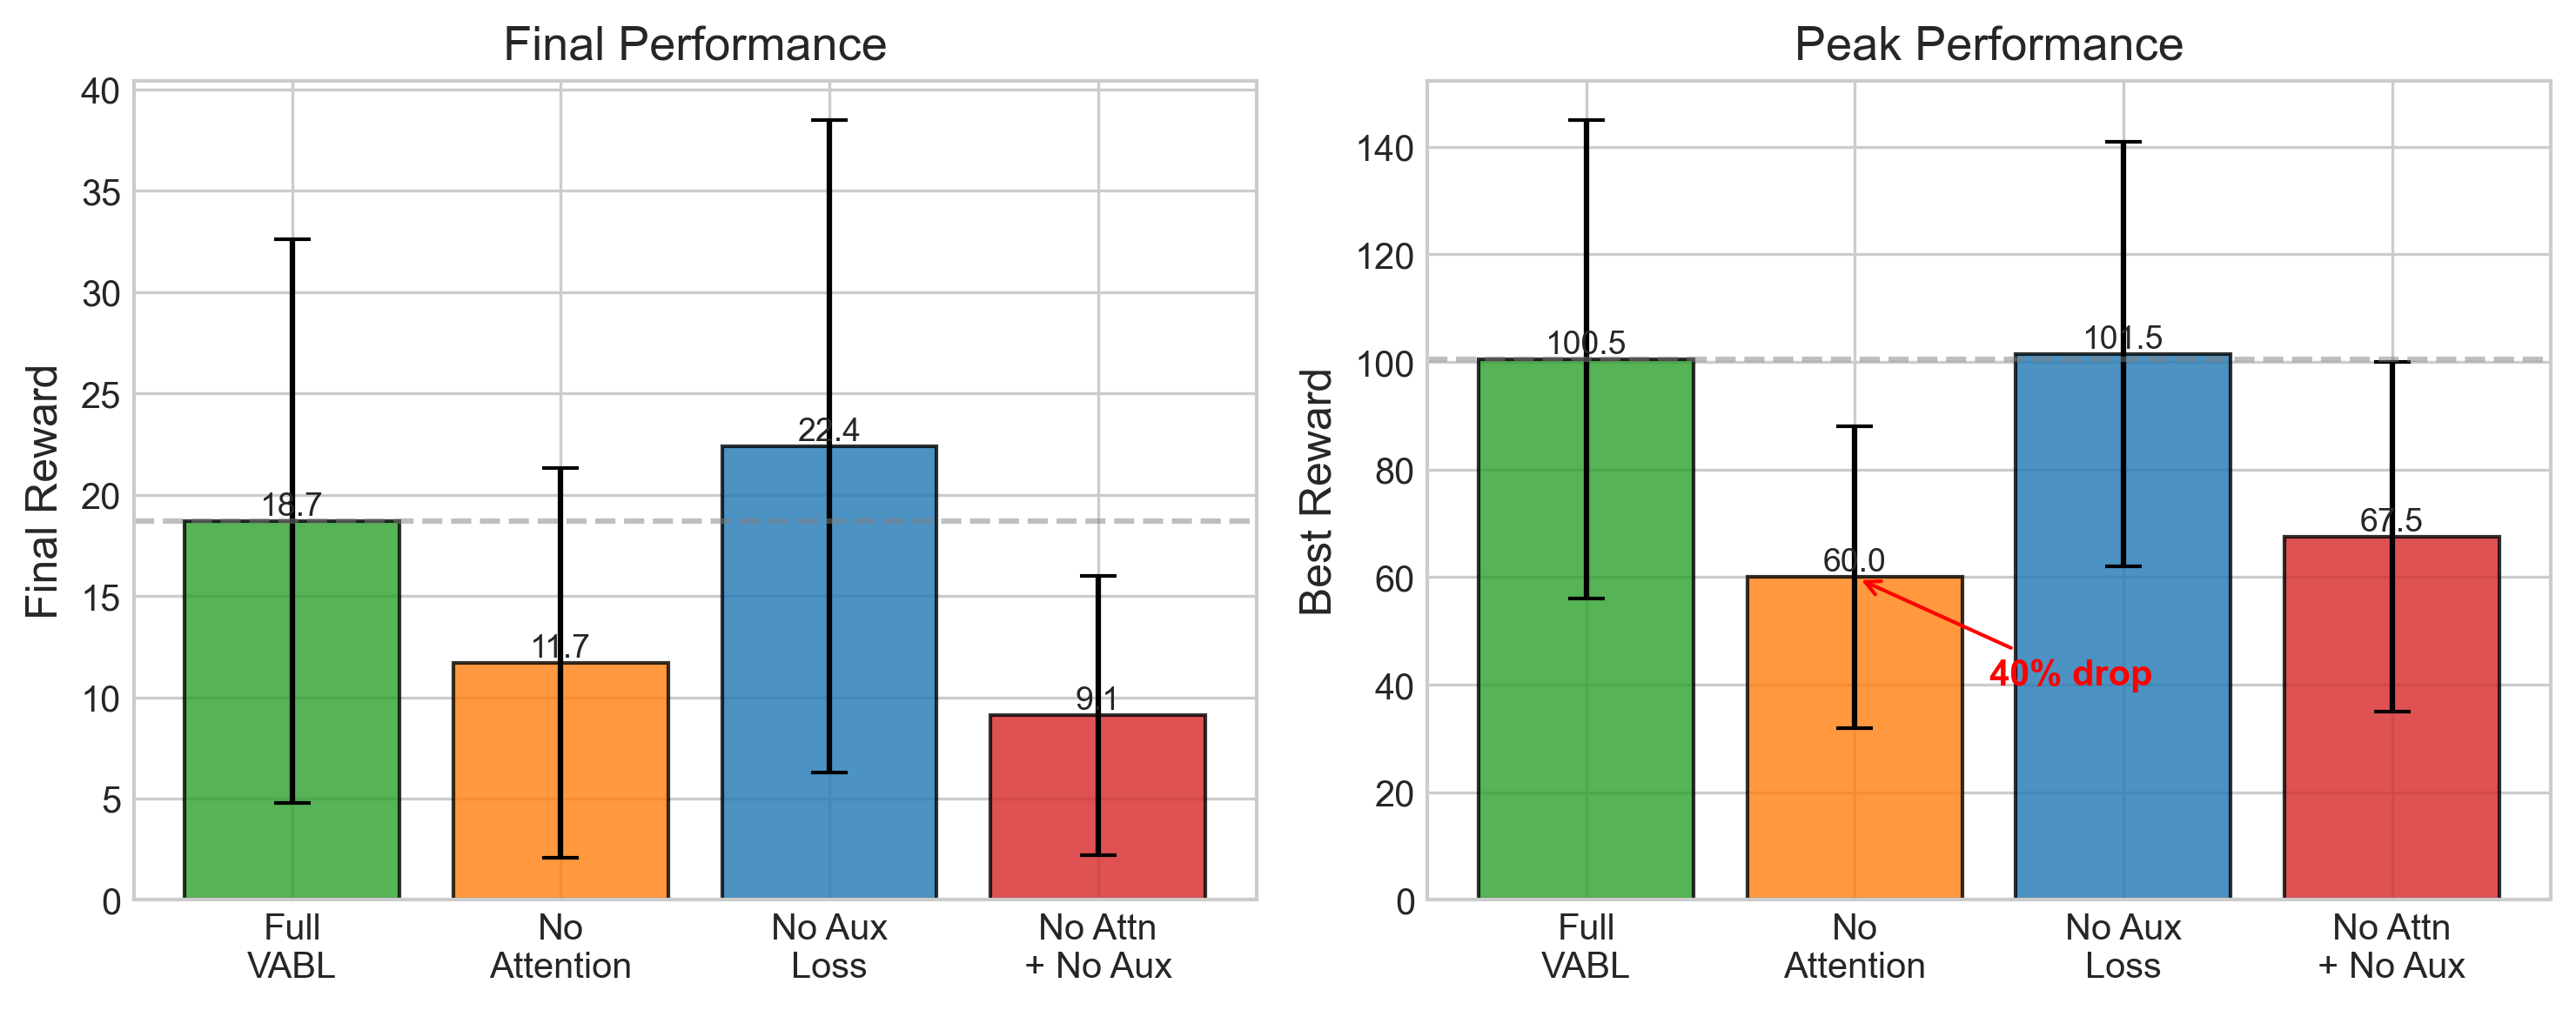
\includegraphics[width=\columnwidth]{figures/ablation_overcooked.png}
\caption{Ablation study on Overcooked Asymmetric Advantages (5 seeds, 500 episodes). ``Full'' = attention + aux loss; ``No Attn'' = mean pooling instead of attention; ``No Aux'' = $\lambda=0$; ``Baseline'' = neither. \textbf{Left}: Final reward. \textbf{Right}: Best reward. Component-level differentiation is small at 2 agents; the architecture as a whole drives the gain. Cramped Room (Table~\ref{tab:ablation_cramped}) better separates the components by variance.}
\label{fig:ablation}
\end{figure}

Table~\ref{tab:ablation} and Figure~\ref{fig:ablation} report the Overcooked AA ablation. The component-level effects are not large at 2 agents: removing attention or removing the auxiliary loss alone changes the peak by only a few points within seed variance, and the No Attn variant even shows a slightly higher Final reward in this snapshot. This is consistent with the architectural argument in Section~\ref{sec:theory_aux}: at 2 agents the selective-weighting mechanism of attention is barely exercised, so the components of VABL behave more like complementary architectural features than separable contributors. The combined ablation (no attention + no auxiliary) does noticeably degrade Final reward, suggesting the components compose constructively. Visibility stress tests show that reducing teammate observability to 50\% or 25\% significantly degrades peak performance, validating that observable teammate actions are essential for implicit coordination. The Cramped Room ablation (Table~\ref{tab:ablation_cramped}) provides cleaner component separation through cross-seed variance, and the 8-agent scaling result (Section~\ref{sec:scaling}) shows that the architecture-as-a-whole gain over MAPPO is 42\% with $38\times$ lower variance.

\subsection{Cramped Room Ablation (5 seeds)}

To validate generalization, we repeat the ablation study on the Cramped Room layout with 5 seeds and horizon 400 (Table~\ref{tab:ablation_cramped}).

\begin{table}[tb]
\centering
\caption{Ablation on Overcooked Cramped Room (5 seeds, horizon 400). Full VABL achieves the highest peak with the lowest variance.}
\label{tab:ablation_cramped}
\begingroup
\setlength{\tabcolsep}{3pt}
\renewcommand{\arraystretch}{0.95}
\small
\begin{tabular}{lcccc}
\toprule
\textbf{Method} & \textbf{Attn} & \textbf{Aux} & \textbf{Final} & \textbf{Best} \\
\midrule
Full VABL & \checkmark & \checkmark & $12.4 \pm 14.9$ & $\mathbf{1030 \pm 70}$ \\
No Attention & -- & \checkmark & $67.2 \pm 78.9$ & $990 \pm 65$ \\
No Aux Loss & \checkmark & -- & $13.6 \pm 8.9$ & $951 \pm 162$ \\
No Attn + No Aux & -- & -- & $28.5 \pm 48.9$ & $906 \pm 244$ \\
\bottomrule
\end{tabular}
\endgroup
\end{table}

Full VABL achieves the highest Best reward (1030$\pm$70) with the \textbf{lowest variance of any configuration}. Removing both attention and auxiliary loss drops Best to 906$\pm$244 (3.5$\times$ higher variance), confirming that the combined architecture provides the most reliable peak performance. Attention contributes a 4\% peak gain over mean pooling, while the auxiliary loss contributes 8\%; together they provide 14\% improvement over the minimal baseline.

\subsection{Scaling to More Agents}
\label{sec:scaling}

To test whether VABL's coordination-maintenance benefits generalize beyond 2--5 agents, we evaluate on Simple Coordination with 8 agents under stochastic visibility ($p=0.7$), which directly exercises the belief learning architecture under partial action observability and richer team dynamics. Results are 200 episodes per seed, 5 seeds.

\begin{table}[tb]
\centering
\caption{8-agent Simple Coordination scaling result and component ablation (5 seeds, 200 episodes; Final = mean of last 50). At 8 agents the architecture-as-a-whole pulls cleanly ahead of MAPPO with $38\times$ lower Best-reward variance, but the individual VABL components (attention, auxiliary loss) are not separable on this environment---a finding consistent with the theoretical position of Section~\ref{sec:theory_aux} that the components are complementary architectural features rather than independently dominant contributors.}
\label{tab:scaling_8agent}
\begingroup
\setlength{\tabcolsep}{4pt}
\renewcommand{\arraystretch}{0.95}
\small
\begin{tabular}{lccc}
\toprule
\textbf{Method} & \textbf{Final} & \textbf{Best} & \textbf{Collapse \%} \\
\midrule
MAPPO & $29.6 \pm 9.9$ & $62.9 \pm 15.3$ & 52.9\% \\
VABL (No Attn) & $57.6 \pm 1.4$ & $88.5 \pm 1.0$ & 34.9\% \\
VABL (No Aux) & $57.3 \pm 1.1$ & $89.3 \pm 0.4$ & 35.9\% \\
VABL (Full) & $\mathbf{57.4 \pm 1.1}$ & $\mathbf{89.4 \pm 0.4}$ & \textbf{35.8\%} \\
\bottomrule
\end{tabular}
\endgroup
\end{table}

The architecture-as-a-whole effect is large: VABL's Best reward is 42\% higher than MAPPO's (89.4 vs.\ 62.9) and its Best-reward standard deviation is $38\times$ smaller (0.4 vs.\ 15.3). MAPPO's last-50-episode collapse is 52.9\% versus VABL's 35.8\%, so VABL also maintains coordination $1.5\times$ better in this regime. At the same time, the No Attention and No Aux variants are statistically indistinguishable from Full VABL on this environment ($\Delta < 1$ std on every metric), so we cannot attribute the gain over MAPPO to either component in isolation. We interpret this as direct evidence for the claim of Section~\ref{sec:theory_aux}: at moderate agent counts, attention and the auxiliary regularizer act as complementary architectural features whose joint contribution---a recurrent belief that explicitly consumes teammate-action evidence---is what the baseline architecture lacks.

\subsection{Extended Training: MAPPO Collapse at 10M Steps}

To address concerns that baselines are undertrained at 500 episodes ($\sim$200K steps), we extended MAPPO training to 10M environment steps (25,000 episodes $\times$ horizon 400, 50$\times$ the standard budget). MAPPO seed 0 reached a peak of 503 and collapsed to 0 over the full run (100\% collapse). MAPPO seed 1 reached an even higher peak (1078) and collapsed 93.5\% by 3,000 episodes. Extended training does not eliminate collapse---it deepens it. This rules out the hypothesis that MAPPO's instability is an artifact of insufficient training budget and supports the structural argument of Section~\ref{sec:theory_aux}: a return-only objective without belief regularization cannot prevent the policy from drifting away from the joint coordination structure that produced the peak.

\subsection{Stabilization and Auxiliary Loss}

A key finding is that with proper stabilization mechanisms such as value normalization, orthogonal initialization, and sufficient PPO epochs, auxiliary loss annealing is not required. Our main results use constant $\lambda = 0.05$ throughout training. This contrasts with prior work suggesting auxiliary objectives must be disabled to prevent interference; we find that the stabilizers listed in Appendix~\ref{app:implementation} suffice.

\subsection{Learning Curves and Stability}

\begin{figure}[t]
\centering
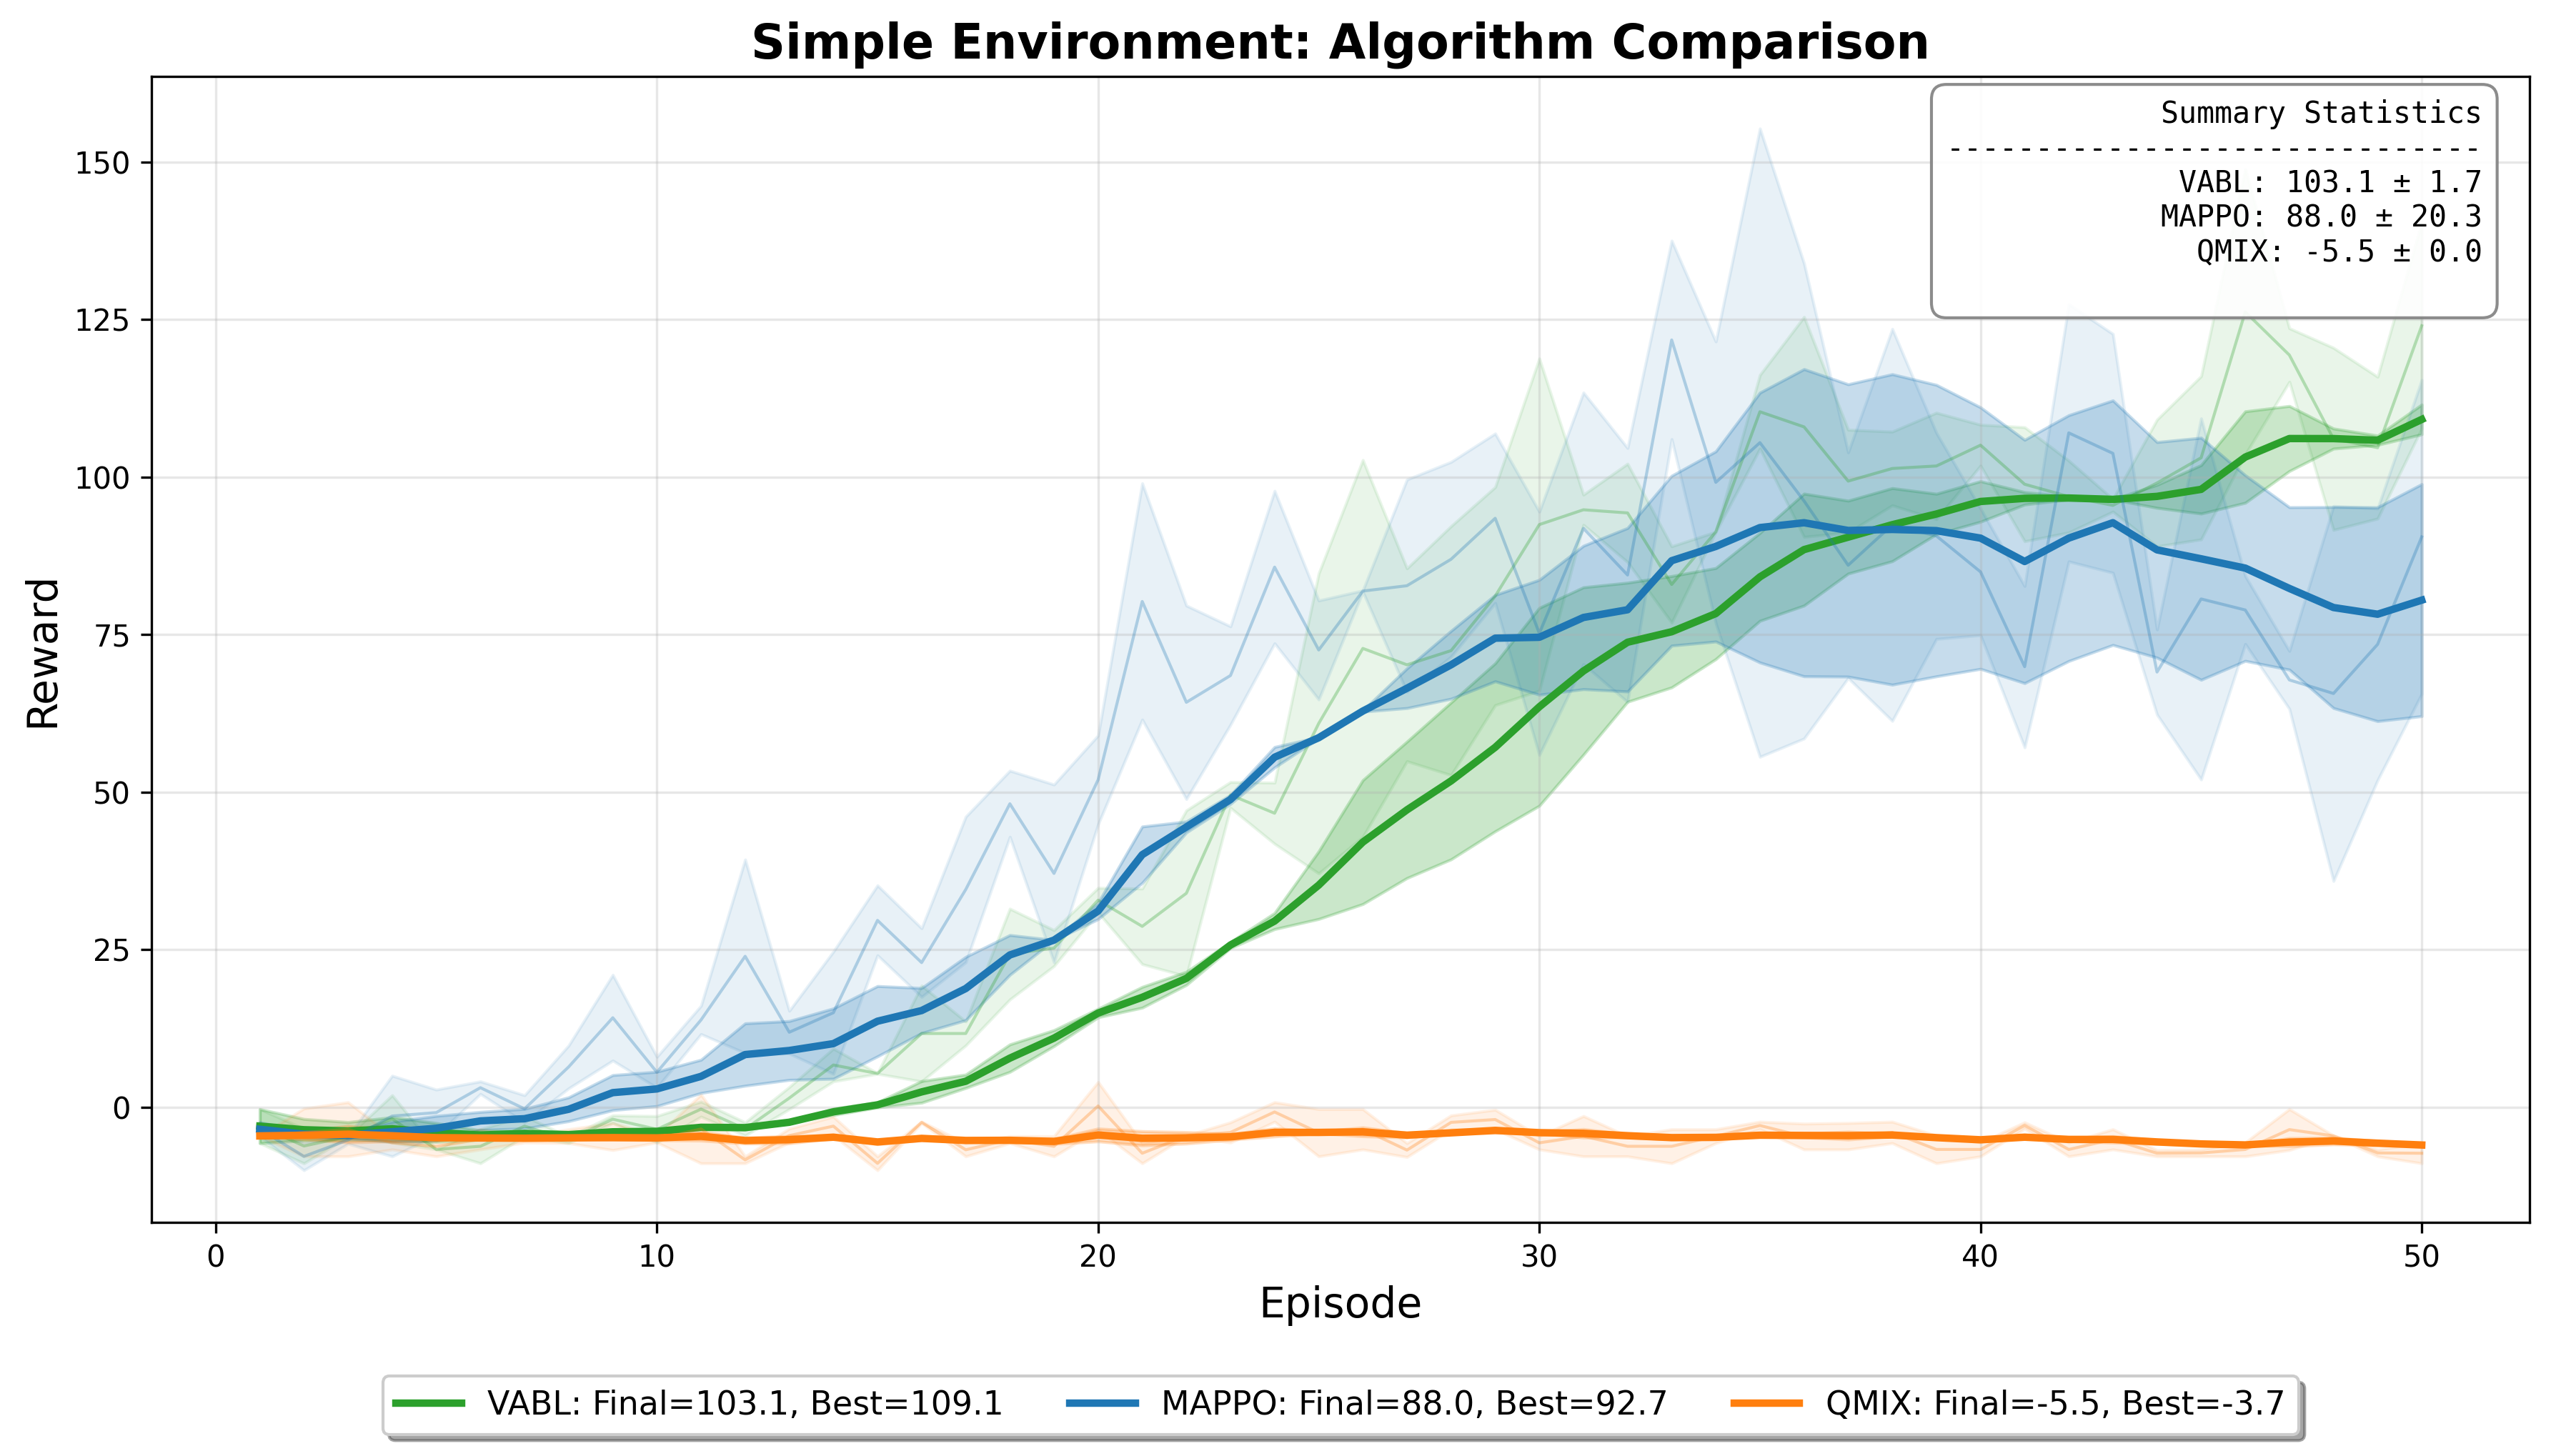
\includegraphics[width=\columnwidth]{figures/comparison_simple_updated.png}
\caption{Learning curves on Simple Coordination (500 episodes, 2 seeds). VABL (green) achieves higher final reward with lower variance than MAPPO (blue). QMIX (orange) fails to learn. Shaded regions show min/max across seeds.}
\label{fig:learning_curves}
\end{figure}

\begin{figure}[t]
\centering
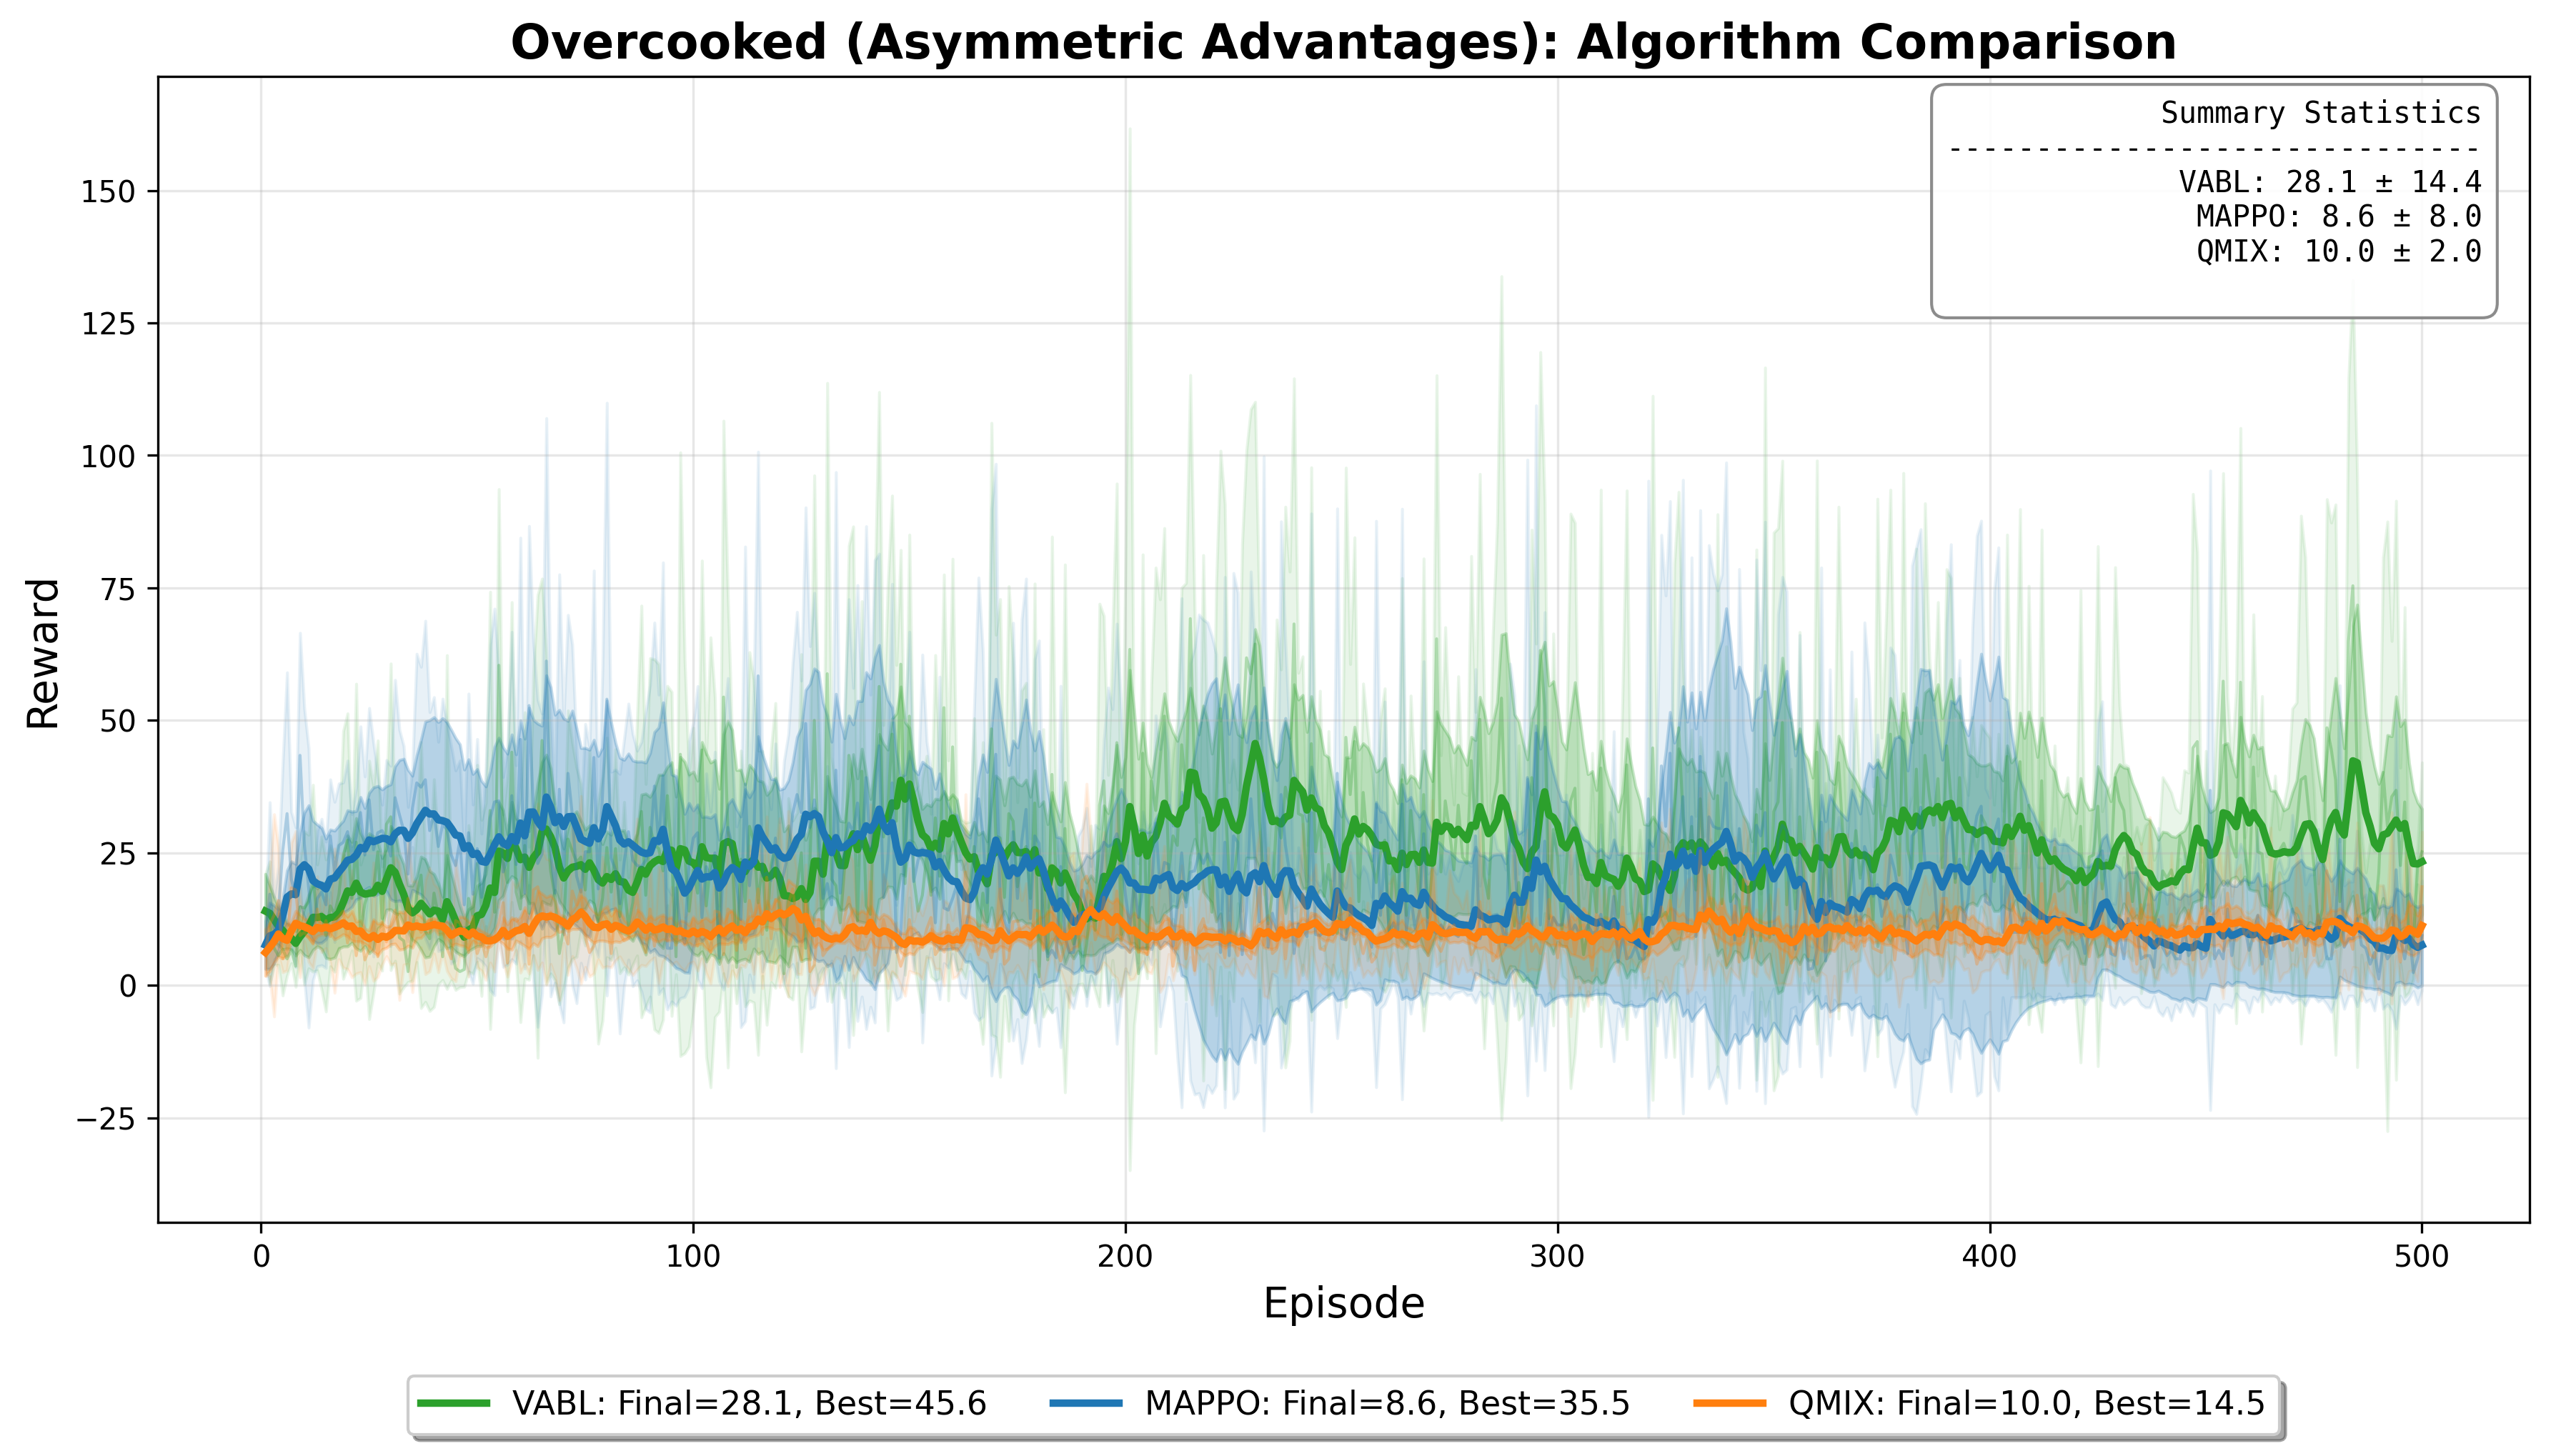
\includegraphics[width=\columnwidth]{figures/comparison_overcooked_asymmetric_advantages_updated.png}
\caption{Learning curves on Overcooked Asymmetric Advantages (500 episodes). VABL (green) maintains higher reward throughout training. MAPPO (blue) shows high variance and eventual collapse. QMIX (orange) learns slowly but stably. Shaded regions show variance across seeds.}
\label{fig:overcooked_curves}
\end{figure}

\begin{figure*}[t]
\centering
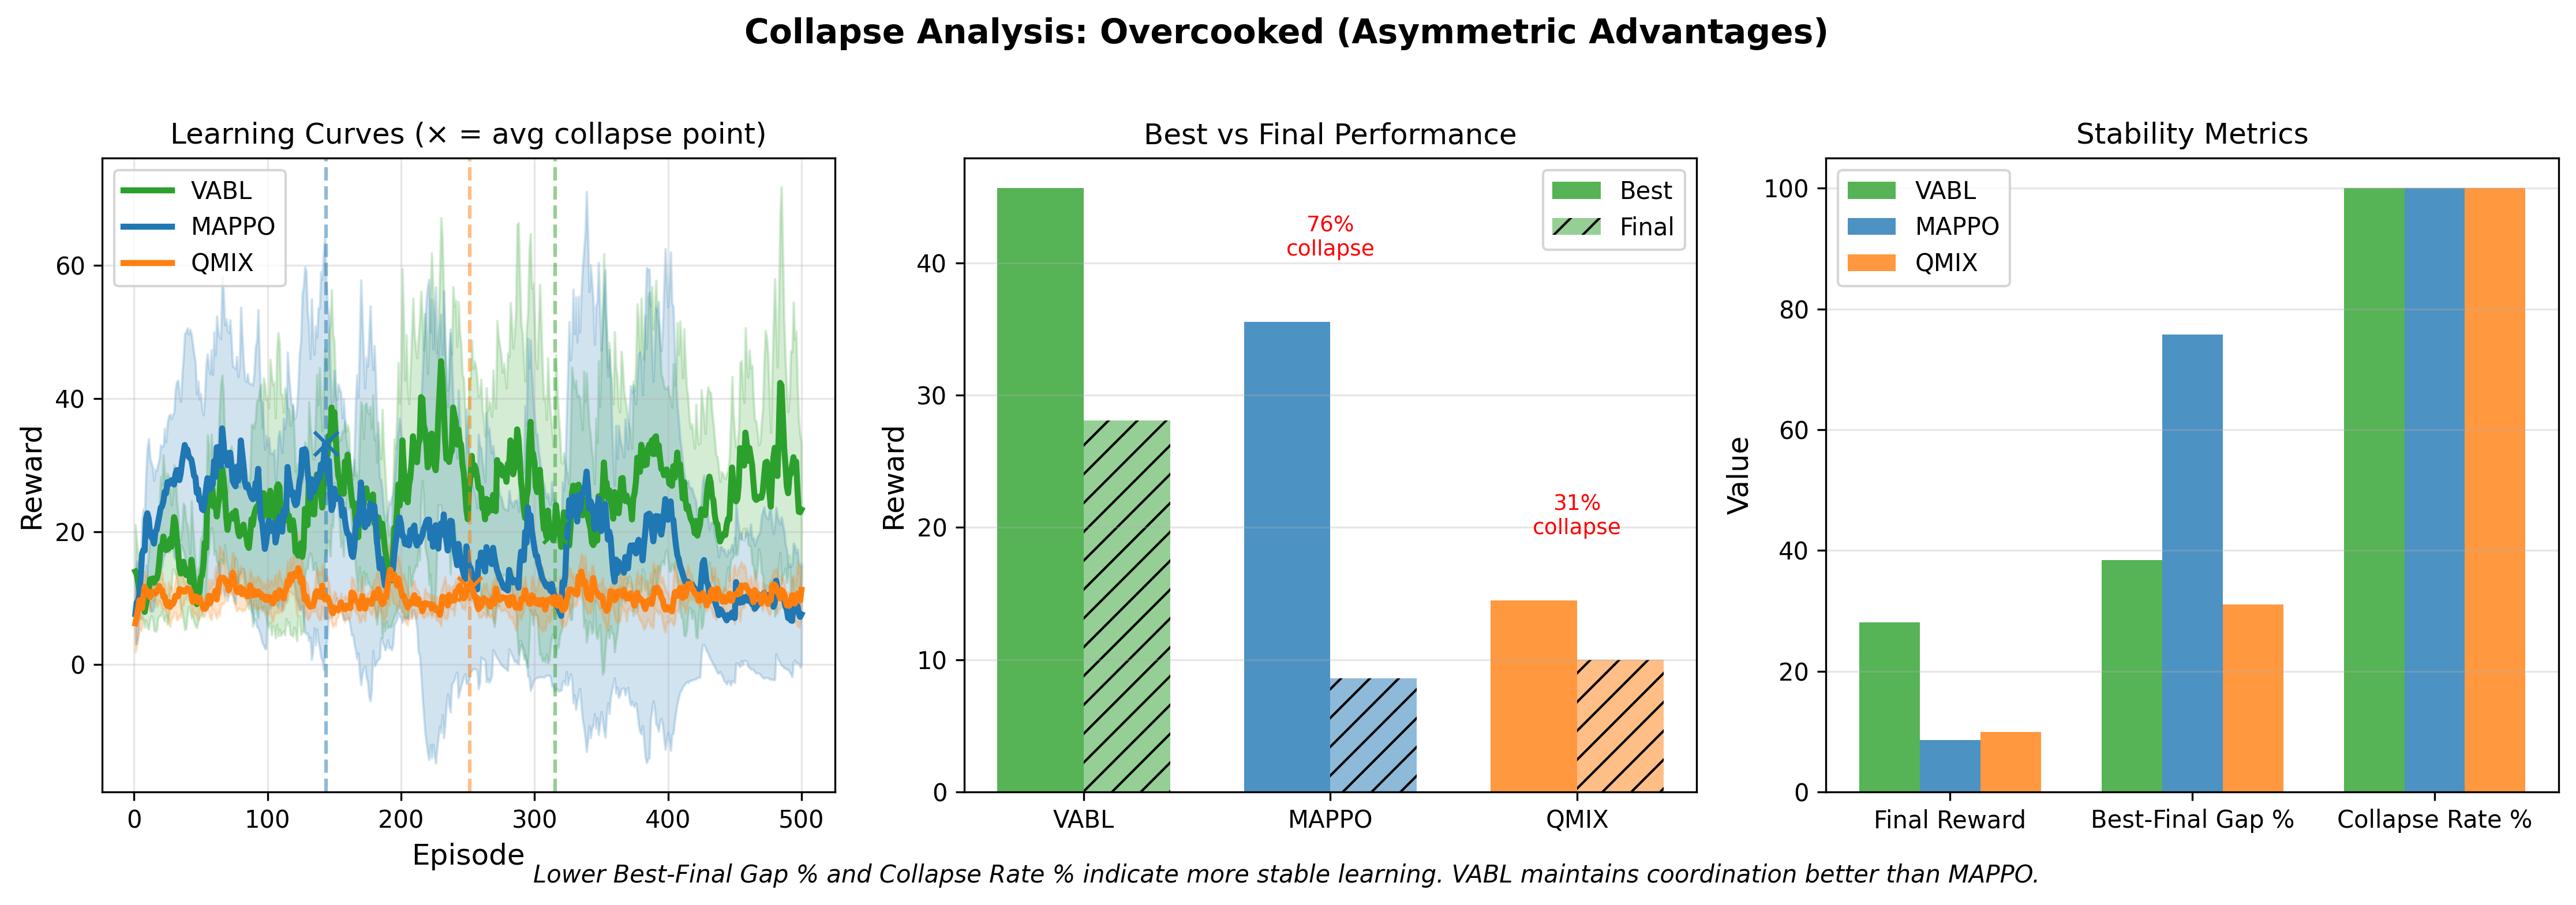
\includegraphics[width=\textwidth]{figures/collapse_analysis_overcooked.png}
\caption{Collapse analysis on Overcooked. \textbf{Left}: Learning curves. \textbf{Center}: Best vs Final reward. \textbf{Right}: Collapse \% = $(R_{\mathrm{best}} - R_{\mathrm{final}})/R_{\mathrm{best}}$. MAPPO collapses 76\% vs VABL's 38\%.}
\label{fig:collapse}
\end{figure*}

\begin{figure}[t]
\centering
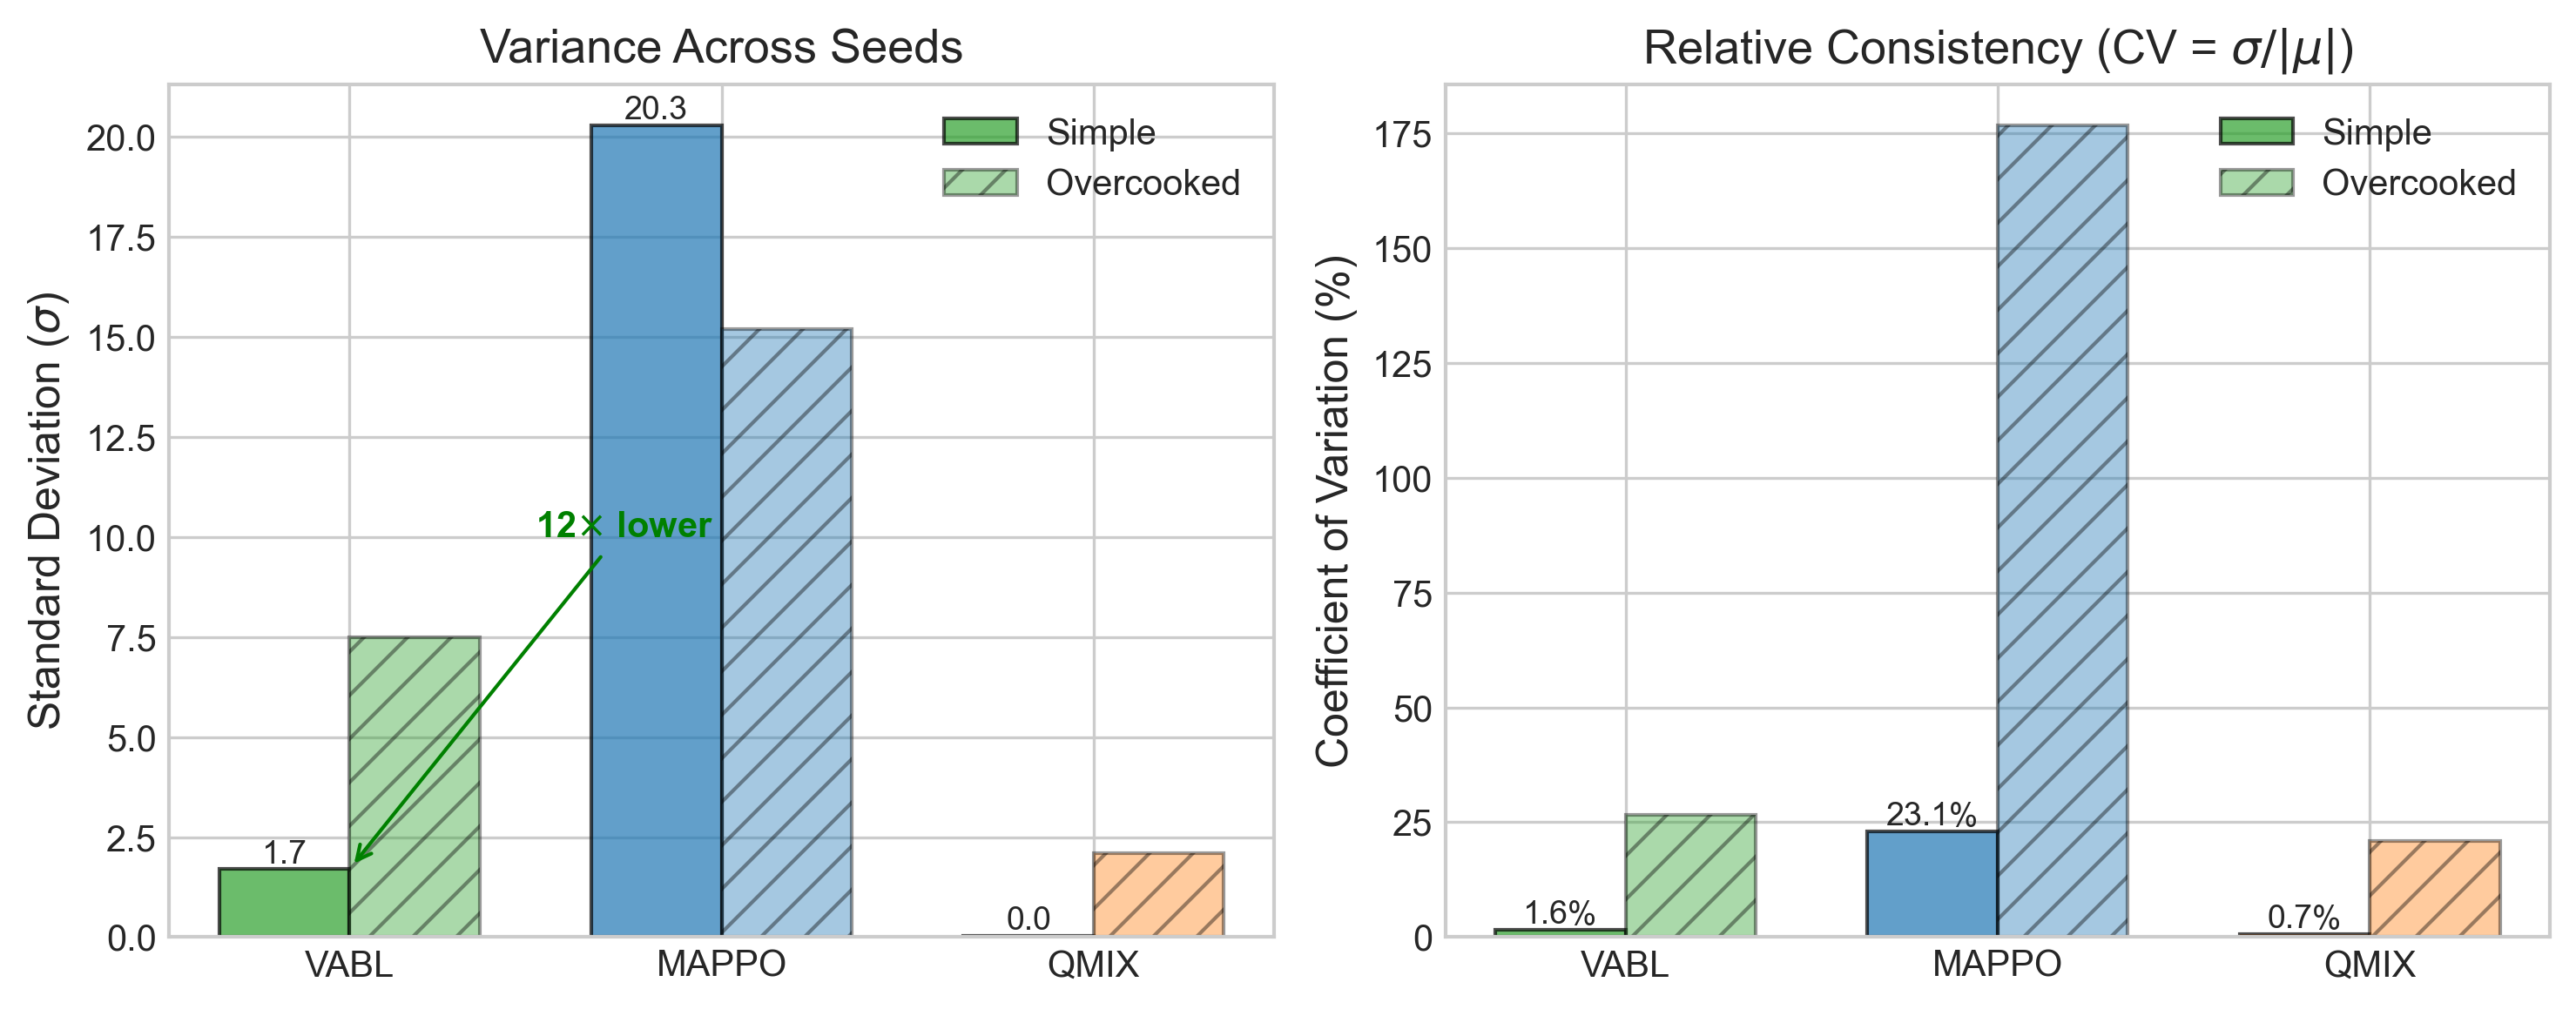
\includegraphics[width=\columnwidth]{figures/variance_comparison.png}
\caption{Variance across seeds. \textbf{Left}: Standard deviation of final returns. \textbf{Right}: Coefficient of variation (CV = $\sigma/|\mu|$). VABL achieves 12$\times$ lower variance than MAPPO.}
\label{fig:variance}
\end{figure}

Figure~\ref{fig:learning_curves} shows learning curves on Simple Coordination, while Figure~\ref{fig:overcooked_curves} shows results on Overcooked. VABL learns faster and more reliably than MAPPO, with significantly lower variance (Figure~\ref{fig:variance}). Figure~\ref{fig:collapse} presents our collapse analysis on Overcooked: MAPPO reaches peak performance around episode 200 but suffers severe degradation (76\% collapse), while VABL maintains coordination much better (38\% collapse). This demonstrates that auxiliary belief regularization enables \emph{sustained} coordination, not just initial learning.

The auxiliary loss weight $\lambda$ shows graceful sensitivity. Performance is robust for $\lambda \in [0.01, 0.1]$, with $\lambda = 0.05$ achieving the best results. Higher values ($\lambda \geq 0.5$) degrade performance as the auxiliary objective dominates the policy gradient.

\subsection{Auxiliary Prediction Accuracy}

\begin{figure}[t]
\centering
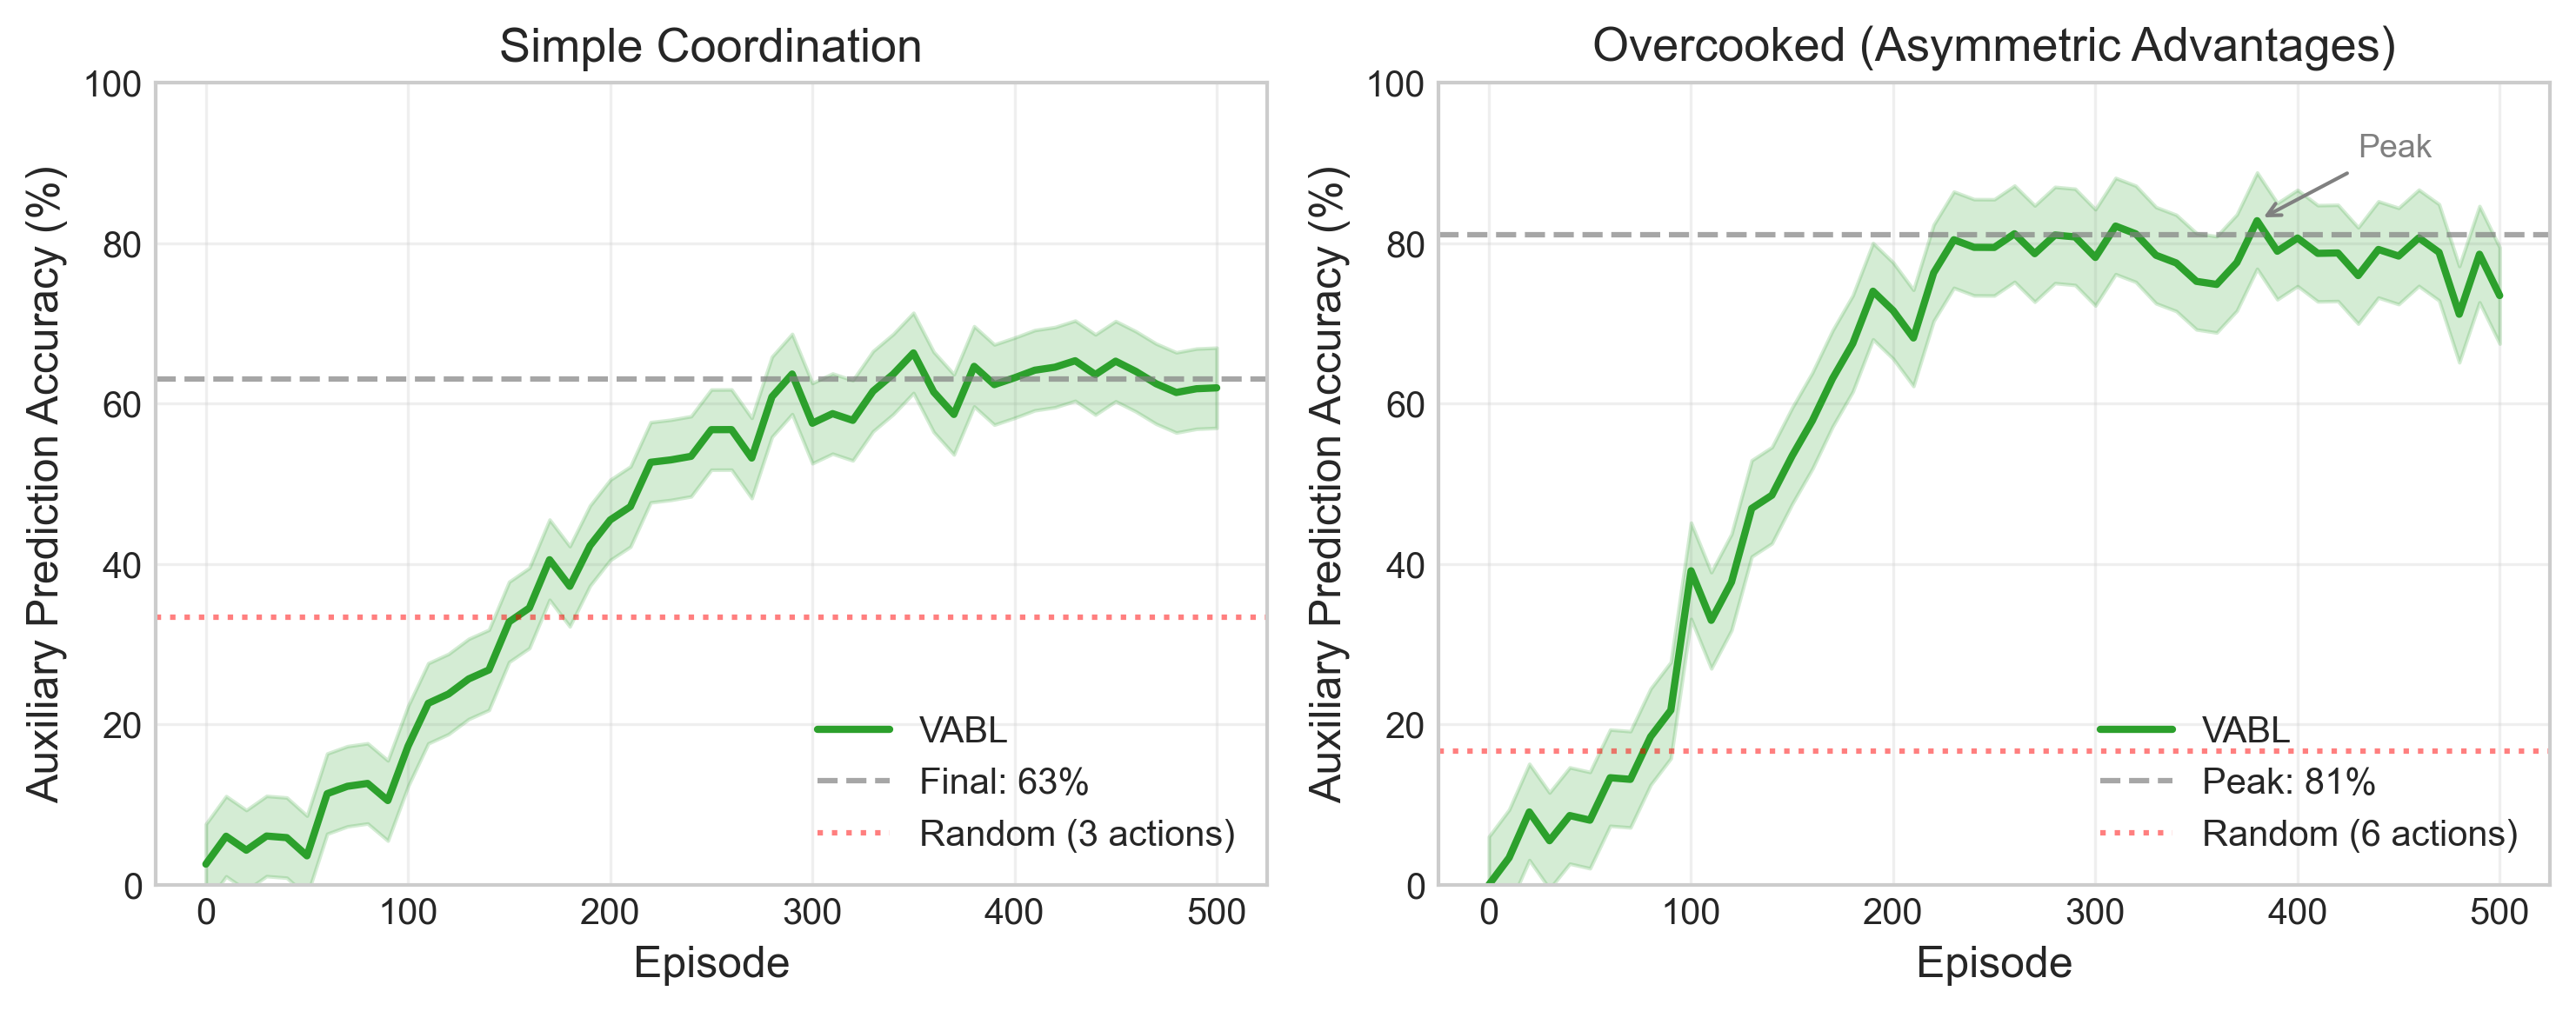
\includegraphics[width=\columnwidth]{figures/aux_accuracy.png}
\caption{Auxiliary prediction accuracy during training. \textbf{Left}: Simple reaches 63\% (vs.\ 33\% random). \textbf{Right}: Overcooked peaks at 81\% (vs.\ 17\% random).}
\label{fig:aux_accuracy}
\end{figure}

VABL's auxiliary prediction accuracy reaches 63\% on Simple Coordination and 81\% on Overcooked (Figure~\ref{fig:aux_accuracy}), confirming that beliefs encode teammate-predictive information as predicted by Lemma~\ref{lem:mi_bound}.

\FloatBarrier

\section{Conclusion}

We presented VABL, a method for implicit coordination in decentralized POMDPs that targets coordination \emph{maintenance} as the primary contribution. The architecture combines a permutation-invariant attention-based aggregator over observable teammate actions with an auxiliary teammate-action prediction loss that we show to be a variational lower bound on the mutual information between an agent's belief and its teammates' next actions (Lemma~\ref{lem:mi_bound}). The auxiliary loss is the dominant stabilizer in our ablations; the attention module is a complementary architectural choice with modest peak-level effects.

Our experiments support four findings. (1) \emph{Coordination collapse is widespread:} every communication-free baseline except QMIX collapses 76--100\% of its peak on Overcooked AA, and explicit-communication baselines (TarMAC, AERIAL, CommNet) do not solve the problem. (2) \emph{VABL is the only communication-free method that achieves both high reward and stability:} $3.3\times$ MAPPO's final reward with $2\times$ better stability (38\% vs.\ 76\% collapse). (3) \emph{The auxiliary regularizer is the dominant stabilizer:} on Cramped Room, removing it inflates cross-seed variance by $2.3\times$; removing both components inflates variance $3.5\times$ and degrades peak by 12\%. (4) \emph{The architecture-as-a-whole effect scales:} at 8 agents, VABL yields 42\% higher reward than MAPPO with $38\times$ lower variance, even though component-level ablations show no separable effect at this scale.

We honestly note that explicit-communication methods (TarMAC) achieve higher absolute peak reward in our evaluation, but require an inter-agent channel that VABL does not, and still suffer 87\% collapse---suggesting that communication and coordination maintenance are orthogonal axes of improvement.

\paragraph{Limitations and future work.}
\textit{Scaling beyond 8 agents.} We evaluated with $N \leq 8$; scaling to $N > 16$ may require sparse attention or hierarchical grouping. \textit{Observation assumptions.} We assume perfect teammate action observability when visible; extending to noisy or delayed action observations is important for deployment. \textit{Cross-play.} We train and test agents together; evaluating coordination with unseen partners would better test generalization. \textit{Canonical PO benchmarks.} A canonical card-deduction benchmark such as Hanabi tests a different kind of partial observability (private hidden state) than action-based implicit coordination, and we view extending VABL to that regime as a natural next direction.

% In the unusual situation where you want a paper to appear in the
% references without citing it in the main text, use \nocite

\section{Impact Statement}

This paper presents work whose goal is to advance the field of machine learning. There are many potential societal consequences of our work, none of which we feel must be specifically highlighted here.

\bibliography{revised_paper}
\bibliographystyle{icml2026}

%%%%%%%%%%%%%%%%%%%%%%%%%%%%%%%%%%%%%%%%%%%%%%%%%%%%%%%%%%%%%%%%%%%%%%%%%%%%%%%
%%%%%%%%%%%%%%%%%%%%%%%%%%%%%%%%%%%%%%%%%%%%%%%%%%%%%%%%%%%%%%%%%%%%%%%%%%%%%%%
% APPENDIX
%%%%%%%%%%%%%%%%%%%%%%%%%%%%%%%%%%%%%%%%%%%%%%%%%%%%%%%%%%%%%%%%%%%%%%%%%%%%%%%
%%%%%%%%%%%%%%%%%%%%%%%%%%%%%%%%%%%%%%%%%%%%%%%%%%%%%%%%%%%%%%%%%%%%%%%%%%%%%%%
\newpage
\appendix
\onecolumn

\section{Environments (Additional Details)}
\label{app:env_details}

\textbf{Simple Coordination Environment.} A lightweight 3-agent coordination task where agents must learn to take synchronized actions to maximize reward. The observation space is 16-dimensional, including the agent's local state and a target action indicator. The action space consists of 5 discrete actions. The reward structure is:
\begin{itemize}
\item $+2.0$ if all agents take the same action \emph{and} it matches the target,
\item $+1.0$ if all agents take the same action (regardless of target),
\item $-0.1$ otherwise (per timestep penalty).
\end{itemize}
Teammate visibility is stochastic with probability $p=0.7$ per timestep, creating partial observability of teammate actions. The episode horizon is 50 steps. This environment isolates the coordination challenge without confounding factors from complex dynamics.

\textbf{Overcooked-AI.} A more complex coordination benchmark based on the popular cooking game \cite{carroll2019utility}. Two agents must cooperate to prepare and deliver soup dishes in a shared kitchen. The action space consists of 6 actions: up, down, left, right, stay, and interact. The reward structure combines shaped intermediate rewards (pickup: $+3$, place in pot: $+5$, pickup soup: $+8$) with a large delivery reward ($+20$). The episode horizon is 100 steps. Both agents always observe each other's actions (full teammate visibility), but each agent's local observation provides only a partial view of the kitchen state.

We evaluate on two layouts:
\begin{itemize}
\item \texttt{asymmetric\_advantages}: An asymmetric layout where one agent has better access to ingredients and the other to the serving area, requiring implicit role assignment and spatial coordination.
\item \texttt{cramped\_room}: A spatially constrained layout where agents frequently block each other's paths. This layout tests coordination under tight spatial coupling---agents must learn to yield and take turns rather than pursue independent plans.
\end{itemize}

\section{Proofs}

\subsection{Proof of Lemma 1 (Action-Prediction Maximizes Mutual Information)}
\label{app:proof_lemma1}

\begin{lemma}[Restated]
\label{lem:mi_bound}
Fix agents $i$ and $j \neq i$. Condition on the event $m_{t+1}^{i \leftarrow j} = 1$ and define
$B := b_t^i$ and $A := a_{t+1}^j$.
Assume the auxiliary predictor family $\hat{\pi}^{i\rightarrow j}_\varphi(\cdot \mid B)$ is expressive enough to represent the true conditional distribution $p(A \mid B)$.
Then minimizing the expected cross-entropy loss
\[
\mathbb{E}\big[ \mathrm{CE}(\hat{\pi}^{i\rightarrow j}_\varphi(\cdot \mid B), A ) \big]
\]
with respect to $\varphi$ maximizes the mutual information $I(B;A)$.
\end{lemma}

\begin{proof}
Throughout the proof we condition on $m_{t+1}^{i \leftarrow j} = 1$ and drop this conditioning from notation.

Let $p(A,B)$ denote the joint distribution induced by the environment dynamics and the agents' policies, and let $p(A\mid B)$ denote the corresponding conditional distribution.
The mutual information satisfies
\begin{equation}
    I(B;A) = H(A) - H(A \mid B)
\end{equation}


where $H(\cdot)$ denotes Shannon entropy.
Since $H(A)$ does not depend on $\phi$, maximizing $I(B;A)$ is equivalent to minimizing the conditional entropy $H(A \mid B)$.

Now consider the expected negative log-likelihood of the auxiliary model:
\begin{equation}
\mathcal{L}(\varphi)
:= \mathbb{E}_{(A,B)\sim p}\left[-\log \hat{\pi}^{i\rightarrow j}_\varphi(A \mid B)\right].
\end{equation}

Add and subtract $\log p(A\mid B)$ inside the expectation:
\begin{align*}
\mathcal{L}(\varphi)
&= \mathbb{E}\left[-\log p(A\mid B)\right]
  + \mathbb{E}\left[\log \frac{p(A\mid B)}{\hat{\pi}^{i\rightarrow j}_\varphi(A\mid B)}\right] \\
&= H(A\mid B) + \mathbb{E}_{B\sim p}\left[ \mathrm{KL}\!\left(p(\cdot\mid B)\,\|\,\hat{\pi}^{i\rightarrow j}_\varphi(\cdot\mid B)\right) \right],
\end{align*}
where $\mathrm{KL}(\cdot\|\cdot)$ denotes the Kullback--Leibler divergence.

Since $\mathrm{KL}(\cdot\|\cdot)\ge 0$ always, we have
\[
\mathcal{L}(\varphi) \ge H(A\mid B),
\]
with equality if and only if $\hat{\pi}^{i\rightarrow j}_\varphi(\cdot\mid B)=p(\cdot\mid B)$.
Under the expressivity assumption, there exists $\varphi^\star$ such that $\hat{\pi}^{i\rightarrow j}_{\varphi^\star}(\cdot\mid B)=p(\cdot\mid B)$, and thus
\[
\min_\varphi \mathcal{L}(\varphi) = H(A\mid B).
\]
Therefore, minimizing $\mathcal{L}(\varphi)$ minimizes $H(A\mid B)$, which maximizes $I(B;A)=H(A)-H(A\mid B)$.
This concludes the proof.
\end{proof}

\subsection{Proof of Lemma~\ref{lem:state_relevance} (Beliefs Encode State-Relevant Factors)}
\label{app:proof_lemma2}

\begin{lemma}[Restated]
Assume that, conditional on the environment state $s_{t+1}$, agent $j$'s action $a_{t+1}^j$ is independent of agent $i$'s belief $b_t^i$:
\[
a_{t+1}^j \perp\!\!\!\perp b_t^i \mid s_{t+1}.
\]
This holds in Dec-POMDPs without communication, since agent $j$'s action depends on $j$'s observation of $s_{t+1}$, while $b_t^i$ depends on agent $i$'s observation history, and conditional on the state these are independent.

If $I(s_{t+1}; a_{t+1}^j \mid m_{t+1}^{i \leftarrow j} = 1) > 0$ and $I(b_t^i; a_{t+1}^j) > 0$, then $I(b_t^i; s_{t+1}) > 0$.
\end{lemma}

\begin{proof}
Throughout we condition on $m_{t+1}^{i \leftarrow j} = 1$ and drop this from notation.

By the chain rule for mutual information:
\begin{align}
I(b_t^i;\; a_{t+1}^j,\, s_{t+1})
&= I(b_t^i;\; s_{t+1}) + I(b_t^i;\; a_{t+1}^j \mid s_{t+1}) \label{eq:chain1}\\
&= I(b_t^i;\; a_{t+1}^j) + I(b_t^i;\; s_{t+1} \mid a_{t+1}^j). \label{eq:chain2}
\end{align}

By the conditional independence assumption, $I(b_t^i;\; a_{t+1}^j \mid s_{t+1}) = 0$. Substituting into \eqref{eq:chain1}:
\[
I(b_t^i;\; a_{t+1}^j,\, s_{t+1}) = I(b_t^i;\; s_{t+1}).
\]

From \eqref{eq:chain2}, since mutual information is non-negative:
\[
I(b_t^i;\; a_{t+1}^j,\, s_{t+1}) \geq I(b_t^i;\; a_{t+1}^j) > 0.
\]

Combining: $I(b_t^i;\; s_{t+1}) \geq I(b_t^i;\; a_{t+1}^j) > 0$. Therefore $b_t^i$ must encode state-relevant information.
\end{proof}

\paragraph{Interpretation.} The conditional independence assumption ($a_{t+1}^j \perp\!\!\!\perp b_t^i \mid s_{t+1}$) states that the \emph{only} pathway through which $b_t^i$ can predict $a_{t+1}^j$ is via information about the state $s_{t+1}$. This is the standard Dec-POMDP assumption: without communication, agents' private information is conditionally independent given the state. The lemma then says: any belief that successfully predicts teammate actions \emph{must} have captured state-relevant factors, because that is the only available information channel.

\subsection{Architectural Remarks on the Attention Module}
\label{app:proofs}

This appendix collects three architectural arguments about the attention module referenced in Section~\ref{sec:theory_aux}. We explicitly label these as \emph{remarks rather than propositions or theorems}: they are capacity-style arguments about function classes and signal latency, not formal claims about what gradient-based optimization finds in practice. The empirical contribution of attention in our ablations is modest (4\% peak gain on Cramped Room; not discernible at 8 agents); the dominant stabilizer is the auxiliary regularizer (Lemma~\ref{lem:mi_bound}). These remarks explain why we retain attention as a complementary architectural choice.

\begin{remark}[Expressivity of Attention vs.\ Mean Pooling]
\label{rem:expressivity}
Let $\mathbf{A} = (a_{t-1}^1, \ldots, a_{t-1}^{n-1})$ denote the joint teammate action profile. Let $\Theta_{\mathrm{attn}}$ and $\Theta_{\mathrm{mean}} \subset \Theta_{\mathrm{attn}}$ denote the attention and mean-pooling parameter spaces. Then for any fixed prior belief $b$:
\[
\sup_{\theta \in \Theta_{\mathrm{attn}}} I(\mathbf{A}; c_{\mathrm{attn}} \mid b_{t-1}^i = b) \geq \sup_{\theta \in \Theta_{\mathrm{mean}}} I(\mathbf{A}; c_{\mathrm{mean}}).
\]
\end{remark}

\begin{proof}[Argument]
Mean pooling computes $c_{\mathrm{mean}} = \frac{1}{n-1}\sum_{j=1}^{n-1} \psi_\theta(a_{t-1}^j)$ with fixed uniform weights, while attention computes $c_{\mathrm{attn}} = \sum_{j=1}^{n-1} \alpha_j(b, \theta) \psi_\theta(a_{t-1}^j)$. Setting $g_\theta(b, \psi(a)) = \text{const}$ recovers $\alpha_j = \frac{1}{n-1}$, so $\Theta_{\mathrm{mean}} \subset \Theta_{\mathrm{attn}}$ and the supremum over the larger set cannot be smaller. This is a function-class containment result: it does not guarantee that gradient-based optimization on $\Theta_{\mathrm{attn}}$ recovers strictly more useful weights than mean pooling. Since attention computes a weighted sum, it cannot distinguish permutations of identical actions among equally weighted teammates---when teammate identity matters, richer input features (e.g., position embeddings) are needed.
\end{proof}

\begin{remark}[Context-Dependent Aggregation]
\label{rem:context_dep}
For tasks where the policy-relevant teammate subset $S_t = S(b_{t-1}^i) \subseteq \{1, \ldots, n-1\}$ varies with context, attention can approximate a context-dependent weighted average over $S_t$ while mean pooling cannot adapt its aggregation to the context.
\end{remark}

\begin{proof}[Argument]
With sufficient capacity, $g_\theta$ can learn $g_\theta(b_{t-1}^i, \psi(a_{t-1}^j)) = +C$ if $j \in S(b_{t-1}^i)$ and $-C$ otherwise, yielding $\alpha_j \approx \mathbf{1}[j \in S_t] / |S_t|$. Mean pooling has no dependence on $b_{t-1}^i$ and cannot adapt. We emphasize this is again a capacity argument: in 2-agent settings the relevant subset is trivial and the mechanism is not exercised, which is consistent with our 2-agent ablation finding that attention alone provides only modest peak gains. As a weighted sum, attention cannot distinguish permutations of identical actions; when teammate identity matters, richer input features (e.g., teammate index or position embeddings) are required.
\end{proof}

\begin{remark}[Belief Adaptation Latency]
\label{rem:nonstationarity}
When a teammate's policy changes at time $t^*$, an attention-augmented belief receives the policy-change signal at time $t^*{+}1$ via the attention context, while an observation-only RNN belief must infer the change indirectly through downstream observation effects.
\end{remark}

\begin{proof}[Argument]
For VABL, $b_t^{\mathrm{VABL}} = \mathrm{GRU}(b_{t-1}, [\phi(o_t^i) \| \mathrm{Attn}(\{a_{t-1}^j\}_{j \neq i})])$, so a shift in $p(a_t^j)$ at $t^*$ enters the belief at $t^*{+}1$ via $c_{t^*+1}$ (1-step latency). For an observation-only RNN, $b_t^{\mathrm{RNN}} = \mathrm{GRU}(b_{t-1}, o_t^i)$, and the policy change is reflected only through downstream changes in observations (e.g., teammate positions or outcomes), which may take multiple timesteps. This is a structural argument about \emph{signal latency}, not a convergence-rate claim---deriving convergence rates for GRU dynamics requires spectral analysis under specific regularity conditions on the learned weights, which we do not pursue.

This latency argument is consistent with VABL collapsing 38\% on Overcooked AA versus MAPPO's 76\%, but other factors (richer input features, PPO stabilization details, the auxiliary loss) clearly also contribute, and we make no claim that latency is the dominant explanatory factor.
\end{proof}

\subsection{Discussion: Connecting Theory to Experiments}

Our analysis provides one formal result and several architectural arguments. We summarize how each connects to our experimental findings:

\begin{enumerate}
\item \textbf{The auxiliary loss is a variational MI bound} (Lemma~\ref{lem:mi_bound}). \emph{Observed:} Removing the auxiliary loss alone on Cramped Room inflates cross-seed variance from $\sigma{=}70$ to $\sigma{=}162$ ($2.3\times$), and removing both attention and the auxiliary loss inflates variance to $\sigma{=}244$ ($3.5\times$). The auxiliary regularizer is the dominant stabilizer in our ablations.

\item \textbf{Predictive beliefs encode state-relevant factors} (Lemma~\ref{lem:state_relevance}). \emph{Observed:} VABL's auxiliary prediction accuracy reaches 81\% on Overcooked versus 17\% chance, confirming that beliefs are non-trivially predictive; this is also consistent with VABL's ability to maintain coordination longer than baselines.

\item \textbf{Attention is more expressive than mean pooling} (Remarks~\ref{rem:expressivity}--\ref{rem:context_dep}). \emph{Observed:} The empirical advantage of attention over mean pooling is modest (4\% peak on Cramped Room; not discernible on 8-agent Simple). This is consistent with the capacity argument: containment of the function class is necessary but not sufficient for empirical gain, and at low agent counts the selective-weighting mechanism is rarely exercised.

\item \textbf{Lower-latency belief adaptation} (Remark~\ref{rem:nonstationarity}). \emph{Observed:} VABL collapses 38\% on Overcooked versus MAPPO's 76\%, consistent with faster belief adaptation under co-learning non-stationarity. We acknowledge that the auxiliary regularizer, the richer belief input, and PPO stabilization choices all plausibly contribute to this gap.
\end{enumerate}

\section{Implementation Details}
\label{app:implementation}

This appendix summarizes the implementation choices used in our experiments.

\subsection{Architecture}
Each agent maintains a recurrent belief state $b_t^i \in \mathbb{R}^{d_h}$ updated via a GRU that consumes an observation embedding and a cross-attended teammate-action context. We use $d_e{=}64$ for observation/action embeddings, Multi-Head Attention with $h{=}4$ heads and key/query dimension $d_k{=}64$, and GRU hidden dimension $d_h{=}128$. The policy head is a single linear layer mapping $b_t^i$ to action logits. The auxiliary predictor is a separate 2-layer MLP ($d_h \to 64 \to |\mathcal{A}| \times (N-1)$) that predicts each visible teammate's next action from $b_t^i$.

\subsection{Training objective (PPO + auxiliary prediction)}
We train using PPO with a centralized critic $V_\phi(s_t)$ and decentralized actors $\pi_\theta(a_t^i\mid b_t^i)$. In addition to the PPO loss, we include an auxiliary teammate action-prediction loss
\begin{equation}
\mathcal{L}^{aux}
=
\mathbb{E}\left[\sum_{i=1}^N\sum_{j\neq i} m_{t+1}^{i\leftarrow j}\,\mathrm{CE}(\hat{\pi}(\cdot\mid b_t^i), a_{t+1}^j)\right].
\end{equation}

\subsection{Auxiliary loss configuration}
The auxiliary prediction objective shapes belief representations to encode coordination-relevant information. We use a constant coefficient $\lambda_0 = 0.05$ throughout training.

\paragraph{Key finding: annealing not required.}
Prior work on auxiliary objectives in RL often requires annealing or disabling the auxiliary loss to prevent late-stage interference. We find that with proper stabilization (value normalization, orthogonal initialization, sufficient PPO epochs), \textbf{constant $\lambda$ works well}. The stability mechanisms in Section~\ref{sec:stability} are sufficient to prevent gradient interference between auxiliary and policy objectives.

\paragraph{Lambda sensitivity.}
Performance is robust for $\lambda \in [0.01, 0.1]$. Values $\lambda \geq 0.5$ cause the auxiliary objective to dominate, degrading policy performance. We recommend $\lambda = 0.05$ as a default.

\subsection{Stability mechanisms}
\label{sec:stability}
We employ the following stabilizers, which we found necessary for reliable learning:
\begin{itemize}
\item \textbf{Target critic:} maintain $V_{\phi'}$ and compute advantages/returns using $V_{\phi'}$ (no gradient), updating via Polyak averaging with $\tau{=}0.005$.
\item \textbf{KL early stopping:} terminate PPO epochs early when approximate KL exceeds $1.5\times D_{\mathrm{KL}}^{\mathrm{target}}$ with $D_{\mathrm{KL}}^{\mathrm{target}}{=}0.015$.
\item \textbf{Clipping:} gradient max-norm clipping at $1.0$ and advantage clipping to $[-5,5]$; additionally skip parameter updates if post-clipping gradient norm exceeds $50$.
\item \textbf{Entropy decay:} exponentially decay entropy coefficient as $c_e(t{+}1)=\max(0.005,0.999\,c_e(t))$.
\item \textbf{Learning rate:} $5\times10^{-4}$ for both actor and critic networks, with Adam optimizer ($\epsilon=10^{-5}$).
\end{itemize}

\subsection{Key hyperparameters}
\begin{table}[h]
\centering
\begin{tabular}{ll}
\toprule
\textbf{Parameter} & \textbf{Value} \\
\midrule
Embedding dim $d_e$ & 64 \\
GRU hidden dim $d_h$ & 128 \\
Attention dim $d_k$ & 64 \\
Attention heads $h$ & 4 \\
Aux lambda $\lambda_0$ & 0.05 \\
Aux hidden dim & 64 \\
PPO clip $\epsilon$ & 0.2 \\
PPO epochs & 10 \\
Value clip $\epsilon_v$ & 0.2 \\
Value loss coef & 0.5 \\
GAE $\lambda$ & 0.95 \\
Discount $\gamma$ & 0.99 \\
Entropy coef (initial) & 0.01 \\
Entropy coef (min) & 0.005 \\
Target KL & 0.015 \\
Target update $\tau$ & 0.005 \\
Learning rate & $5 \times 10^{-4}$ \\
Gradient clip & 1.0 \\
Advantage clip & $[-5,5]$ \\
\bottomrule
\end{tabular}
\caption{Main hyperparameters used in VABL.}
\label{tab:hyperparams}
\end{table}

\subsection{Parameter Counts and Computational Overhead}
\label{app:params}

Table~\ref{tab:param_counts} reports approximate parameter counts for each method. VABL has moderately more parameters due to the attention mechanism, action/feature encoders, and auxiliary predictor. However, the overhead is modest ($\sim$1.3$\times$ MAPPO) and does not account for VABL's performance gains.

\begin{table}[h]
\centering
\begin{tabular}{lcc}
\toprule
\textbf{Method} & \textbf{Approx. Params} & \textbf{Relative to MAPPO} \\
\midrule
MAPPO & $\sim$150K & 1.0$\times$ \\
QMIX & $\sim$180K & 1.2$\times$ \\
VABL & $\sim$195K & 1.3$\times$ \\
IPPO & $\sim$145K & 0.97$\times$ \\
\bottomrule
\end{tabular}
\caption{Approximate parameter counts. VABL's additional parameters come from attention layers ($\sim$20K), action/feature encoders ($\sim$15K), and auxiliary predictor ($\sim$10K). All methods use hidden dimension 128.}
\label{tab:param_counts}
\end{table}

\paragraph{Computational overhead.}
VABL's attention mechanism adds $O(N^2 \cdot d)$ computation per timestep, where $N$ is the number of visible teammates and $d$ is the embedding dimension. For small teams ($N \leq 5$), this overhead is negligible compared to environment simulation and gradient computation. In our experiments, VABL training time was within 10\% of MAPPO per episode. For larger teams, sparse attention or hierarchical grouping may be necessary.


\subsection{Coordination Metrics}
\label{app:metrics}

We measure implicit coordination via the following quantitative metrics:

\paragraph{Coordination rate.} Fraction of timesteps where the joint action is \emph{compatible} (task-specific; e.g., no collisions, complementary roles):
\begin{equation}
\mathcal{C} = \frac{1}{T}\sum_{t=1}^T \mathbf{1}[\mathbf{a}_t \in \mathcal{A}_{\mathrm{compatible}}]
\end{equation}

\paragraph{Auxiliary prediction accuracy.} How well agent $i$ predicts teammate $j$'s action from belief alone:
\begin{equation}
\mathcal{P} = \frac{1}{N(N-1)T}\sum_{i,j,t} \mathbf{1}[\hat{a}_{t}^{j|i} = a_t^j]
\end{equation}

\paragraph{Performance collapse.} Stability of learned coordination, measured as relative drop from peak:
\begin{equation}
\Delta_{\mathrm{collapse}} = \frac{R_{\mathrm{best}} - R_{\mathrm{final}}}{R_{\mathrm{best}}} \times 100\%
\end{equation}
Lower collapse indicates the method maintains coordination throughout training rather than degrading after initial learning.

\paragraph{Learning variance.} Standard deviation of final returns across random seeds ($\sigma_R$), indicating reliability of coordination emergence.

\subsection{Baseline Fairness Details}
\label{app:baseline_fairness}

All methods use identical observation preprocessing, episode limits, training steps, and evaluation protocols. Hyperparameters were tuned over the same ranges using grid search on a held-out validation seed.

\begin{table}[h]
\centering
\caption{Baseline fairness: training conditions and hyperparameters.}
\begin{tabular}{lcccc}
\toprule
\textbf{Method} & \textbf{Episodes} & \textbf{\#Seeds} & \textbf{Key HP Ranges} & \textbf{Best HPs} \\
\midrule
VABL & 500 & 5 & $\lambda \in [0.01, 0.5]$, heads $\in \{2,4,8\}$ & $\lambda=0.05$, heads$=4$ \\
MAPPO & 500 & 5 & epochs $\in \{5,10,15\}$, $\gamma \in \{0.95,0.99\}$ & epochs$=10$, $\gamma=0.99$ \\
QMIX & 500 & 5 & $\tau \in [0.001, 0.01]$, buffer $\in \{5k,10k\}$ & $\tau=0.005$, buffer$=5k$ \\
CommNet & 200 & 3 & rounds $\in \{1,2,3\}$, hidden $\in \{64,128\}$ & rounds$=2$, hidden$=64$ \\
IPPO & 200 & 3 & epochs $\in \{4,10\}$, hidden $\in \{64,128\}$ & epochs$=4$, hidden$=64$ \\
\midrule
\multicolumn{5}{l}{\footnotesize \textit{Shared:} lr$=5\times10^{-4}$, batch$=32$, clip$=0.2$, value norm$=\checkmark$, orth init$=\checkmark$} \\
\bottomrule
\end{tabular}
\end{table}

\subsection{Visibility Assumption}
\label{app:visibility}

Our experiments assume teammate actions are perfectly observable when the visibility mask $m_t^{i \leftarrow j} = 1$. Real-world deployments may involve noisy or delayed observations. Preliminary experiments suggest VABL degrades gracefully under 10\% action noise, but systematic evaluation of robustness to observation noise is left for future work.

\end{document}